In this chapter we describe a software framework called Rheos, which demonstrates an approach for reasoning about large genomic datasets utilizing concepts of service-orientation and data streaming in contrast with traditional genomic data analysis frameworks\autocite{depristo2011framework} that take a procedural batch-based approach. Rheos' focus on service-orientation and streaming allow the users to make active tradeoff decisions between analysis time, cost, and quality as well as setting up precise operational Service Level Agreements, both between Rheos components, and between Rheos and external systems, as we describe in detail below.

\section{General Framework Design}

As already discussed in Chapters \ref{ch:introduction} and \ref{ch:background}, the general problem consists of collecting DNA samples from a population of individuals under study, sequencing these samples using Next Generation Sequencing techniques, identifying the mutations that are present, annotating their functional impact and utilizing the obtained data in a downstream data analysis with research or clinical decision-making goals. While there is a great variety of possible downstream analyses that may be performed depending on the individual goals of the analyst, there is a fairly well established set of steps for processing of the raw NGS data into a set of annotated variants, and it is these steps that we target with this work. The typical approach that is in widespread use today is to collect a batch of samples and then process each sample individually with a sequence of individual tools, that may be described via a higher-level workflow construct (such as in Figure \ref{fig:gatk_best_practices}, or using a framework like Butler, as described in Chapters \ref{ch:butler_architecture}, \ref{ch:butler_implementation}). There are, however, a number of factors that leave room for improvement in this model. These improvements lie along a set of dimensions that we describe briefly in the Introduction via a utility function $U_i = C_i + T_i + A_i$ for sample $i \in [1,N_s]$  that needs to be optimized, and that we describe in more detail here.

We use the following definitions throughout the text:

\begin{table}[!ht]
    \caption{Rheos common definitions}
    \label{tab:rheos_notation}
    {\begin{tabular}{lp{7cm}}
    \toprule
    Symbol & Description \\
    \midrule
    $N_p$ & Number of people \\
    $P = \{p_i : i \in [1,N_p]\}$ & Set of individuals under study \\
    $N_s$ & Number of samples \\
    $S = \{s_i : i \in [1,N_s]\}$ & Set of sequenced DNA samples. Each individual can have one or more samples. \\
    $A_i $ & Accuracy score of analysis for sample $i$ (precise definition of Accuracy TBD) \\
    $C_i = c_{g_i} + c_{s_i} + c_{a_i} + c_{r_i}$ & Cost score of data generation, storage, analysis, and retrieval respectively \\
    $T_i$ & Time score to process sample $i$ \\
    $U_i = C_i + T_i + A_i$ & A utility function for individual $i$ that penalizes high cost, high processing time, and low accuracy\\
    $U = \sum_{i=1}^{N_s} U_i$ & Overall utility of processing $N_s$ samples through Rheos.\\
    \bottomrule
    \end{tabular}}
\end{table}


\section{Data Streaming Architecture}
\label{sec:rheos_streaming_architecture}

The overall technical architecture of the Rheos system is set up as a Service Oriented Architecture (SOA)\autocite{shaw1996software} which is an information system architecture paradigm where the overall problem that the system is trying to solve is broken down into a collection of loosely-coupled components called services. Each service has a well defined interface of inputs that it accepts and outputs that it produces. Services can be combined and orchestrated together to produce the overall desired output for the system. A key distinguishing feature of this architectural approach is that each service can be individually optimized to fulfill its contract most efficiently helping break down some of the performance limitations brought about by the necessity to simultaneously tackle competing constraints in more monolithic information system designs. Additionally, within a services framework, the dependencies between separate services can be negotiated not only in terms of service interfaces, but also in terms Service Level Agreements which constitute Quality of Service promises made by one service to its dependents\autocite{ingham2000constructing}. Because it is unlikely that a service designer will be able to accurately foresee all of the demands that will be placed on a service during its lifetime the SLAs provide a valuable feedback framework through which the service can be evaluated as it operates in production, as well as serving as a basis for negotiating evolving requirements between dependent services.

While general web services can support any data processing paradigm, in the Rheos framework we adopt a data streaming approach\autocite{babcock2002models}. In this approach we assume that the input to any service is a randomly ordered sequence of messages $M = {m_1, m_2, ....}$ where each message represents a fact about the underlying domain that the service reasons over, as well as some metadata, including an identifier, and a variety of timestamps of interest. The content of each message may provide a datum, such as the measurement of a quantity of interest, or signal that a particular event has taken place. It is in general assumed that the data stream is infinite in size, that messages may arrive out of order, and that any message that is placed in the stream is observed at most once, and may, in fact, never be observed. Messages are typically not sent directly from one service to another, instead the transfer of messages is mediated by a queuing system using a publish-subscribe\autocite{eugster2003many} model. Under this model each queue acts as a \emph{topic}. Message producers can publish data to the topic, and message consumers subscribe to receive messages from the topic. A message is consumed from the queue only after all of the subscribed consumers have seen it. End users retrieve information from the system via a set of User Interfaces that support both push (notifications) and pull (querying) models of data retrieval. A more detailed description of the architectural aspects of the system follows:

\subsection{Service-Oriented Data Streaming Model}
\label{sec:rheos_data_streaming_model}


A data stream $M_{s,d} = {m_1, m_2, ....}$ is a sequence of datagrams transmitted over the network with the following properties:

\begin{itemize}
    \item The stream has a source $s$ and a destination $d$.
    \item A message $m$ in the stream is a tuple of the form $(header, payload)$, where:
    \begin{itemize}
        \item $header$ is a tuple of the form $(id, \dots)$ that holds at minimum a unique identifier $id$ for messages, and may hold additional metadata.
        \item $payload$ is an arbitrary data structure that holds the informational content of the message. 
    \end{itemize}
    \item $|M| = \infty$ by assumption.
    \item Messages may not arrive at destination $d$ in the same order that they were sent from source $s$.
    \item If $t_{i,s}$ is the time message $m_i$ leaves the source $s$ and $t_{i,d}$ is the time of arrival at destination $d$, then $\sup_i \{t_{i,d} - t_{i,s}\} = \infty$, i.e. a given sent message may never arrive at its destination.
\end{itemize}

A service $S = \{o_i\}$ is a collection of operations $o_i$ that act on one or more input data streams $\{M_i\}$ to produce one or more transformed output data streams $\{M_j\}$. Specifically:

An operation $O$ is a tuple of the form:

\begin{equation}
\label{eq:service_opertaion_equation}
O = (i,o,p,f)
\end{equation} 
where:
\begin{itemize} 
    \item $i = \{M_j, j \in [0, K]\}$ is a set of $K \ge 0$ input data streams.
    \item $o = \{M'_j, j \in [0, L]\}$ is a set of $L \ge 0$ output data streams.
    \item $f:M^K \mapsto M'^L$ is a transformation function that produces messages $m'$ in the output streams based on messages $m$ observed in the input streams.
    \item $p = \{p_i\}$ is a set of potentially optional query parameters.  
\end{itemize}

There are several distinct categories of operations that a service can perform on a set of input streams. We describe these here:

\paragraph{Windowing Function} - Service $S$ observes a sliding window, which is a sample of size $n$ of messages from stream $M_i$ and computes a summary statistic (see Figure \ref{fig:stream_window_function}) over the sample which is meant to be an approximation of the corresponding population parameter.

\begin{figure}[H]
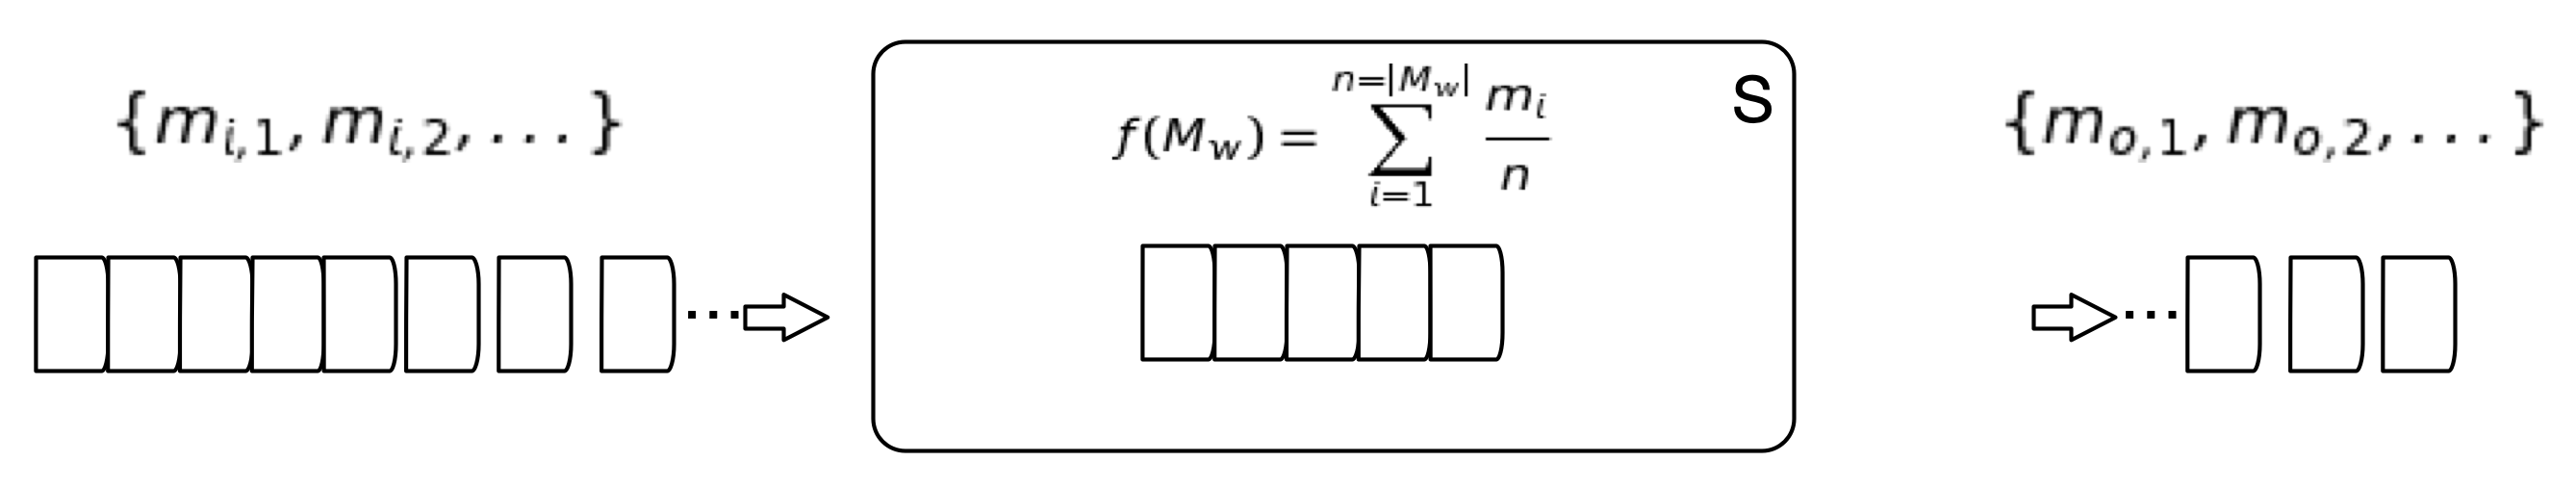
\includegraphics[scale=0.6]{stream_window_function}
\centering
\caption {Service S computes a summary statistic over a window of messages from stream $M$}
\label{fig:stream_window_function}
\end{figure}
 
\paragraph{Decorator Function} - Service $S$ observes messages $m_i$ and applies a function that augments (decorates) each message with additional attributes (see Figure \ref{fig:stream_decorator_function}) producing augmented messages $m_o$ as output.

\begin{figure}[H]
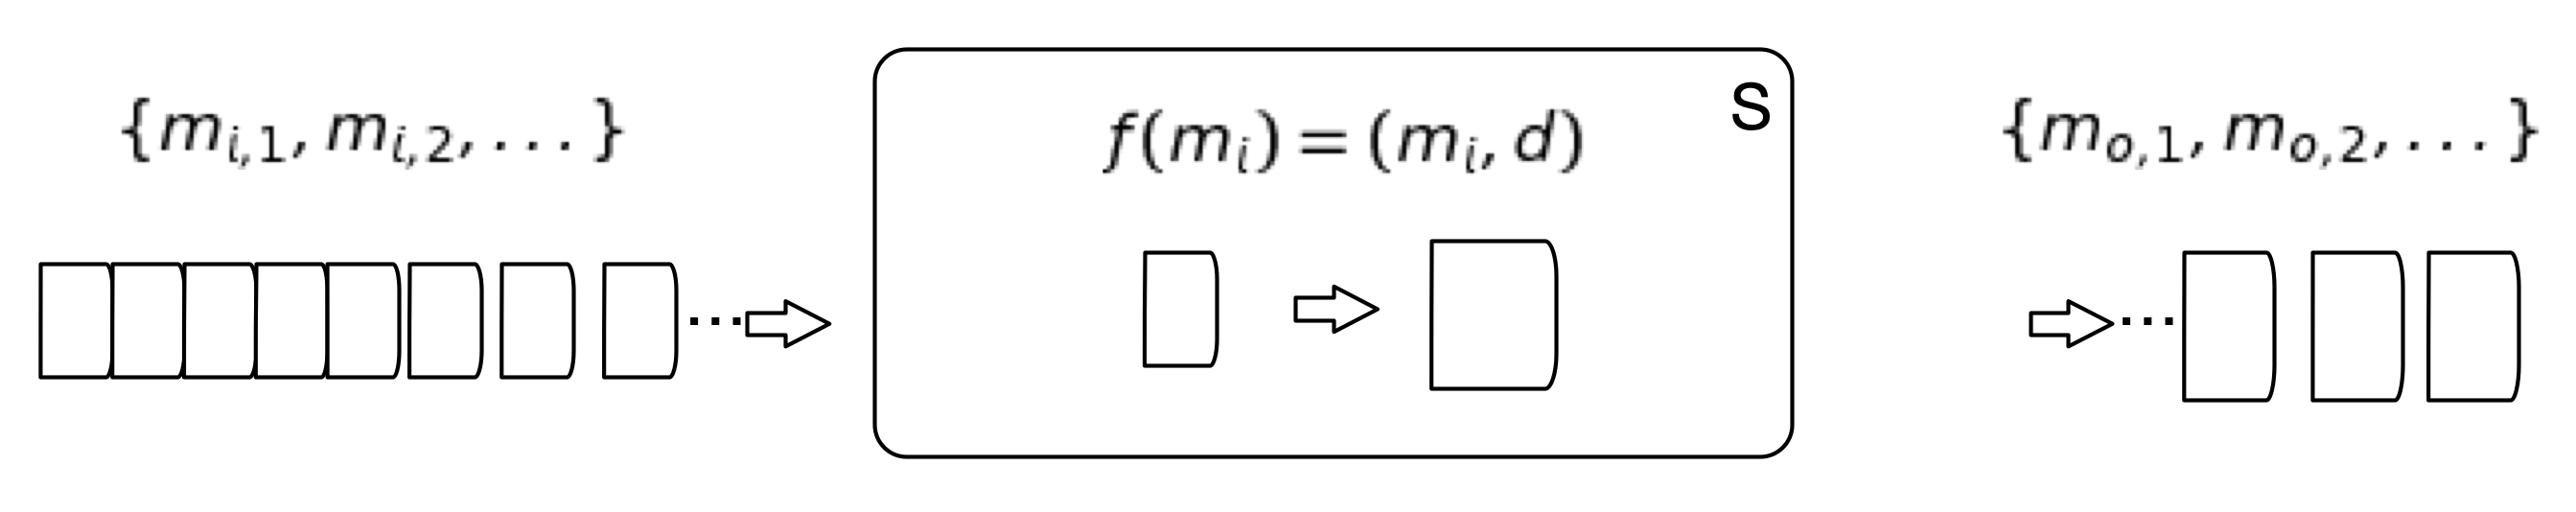
\includegraphics[scale=0.6]{stream_decorator_function}
\centering
\caption {Service S augments messages from $M$ with an additional set of attributes.}
\label{fig:stream_decorator_function}
\end{figure}

\paragraph{Filter Function} - Service $S$ observes messages $m_i$ and applies a function $f:M\mapsto\{True,False\}$ that evaluates to a boolean value (see Figure \ref{fig:stream_decorator_function}). Only messages that map to $True$ are emitted as output.

\begin{figure}[H]
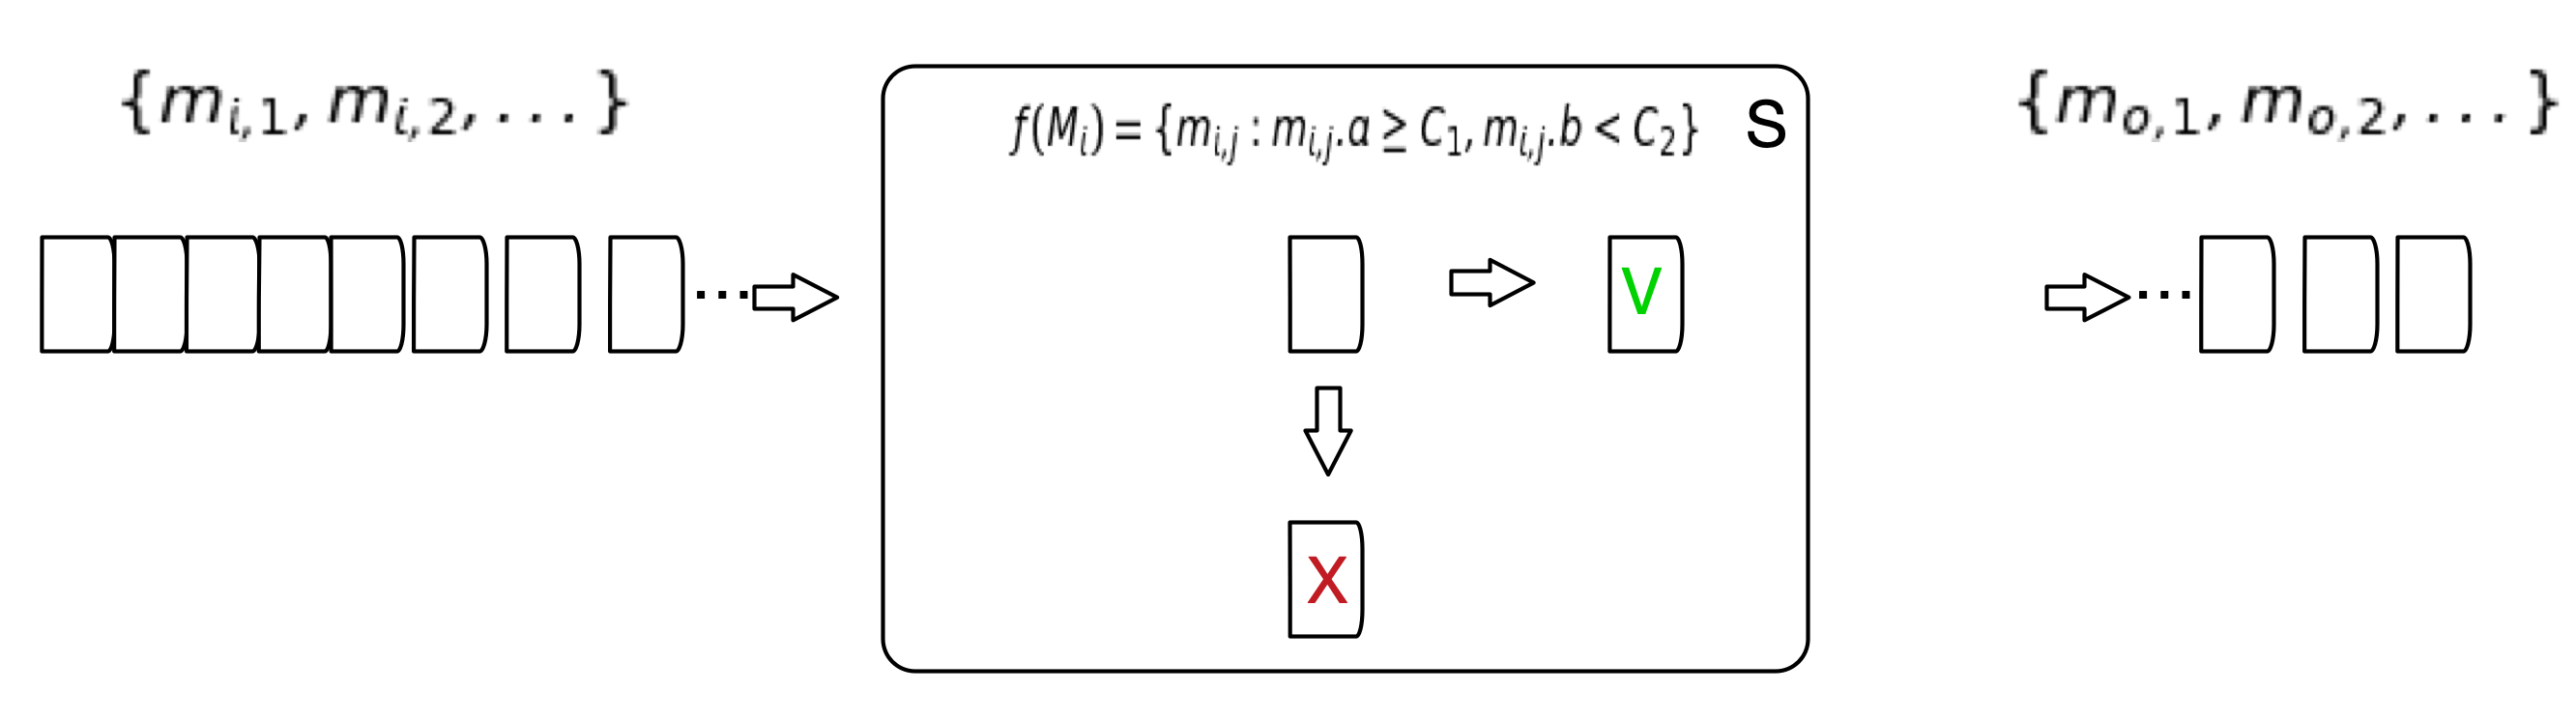
\includegraphics[scale=0.6]{stream_filter_function}
\centering
\caption {Service S filters messages from input stream $M$ and only allows through those that pass the filtering condition.}
\label{fig:stream_filter_function}
\end{figure}

\paragraph{Aggregator Function} - Service $S$ observes messages from $N$ different streams $\{M_j: j \in [1,N]\}$ and applies a function $f:M_i^N \mapsto M_o$ that aggregates messages from these streams to produce its output (see Figure \ref{fig:stream_aggregator_function}). Because aggregation happens over groups of messages that may not all arrive at the same time the service $S$ requires a mechanism for keeping local state so that it can accumulate messages that have already arrived while waiting for those that are necessary to compute $f$ yet have not been observed. The statefulness requirement of this type of service places an extra level of complexity (related to state-management and request routing) as well as inherent scalability limitations compared to stateless services\autocite{oppenheimer2002architecture}.

\begin{figure}[H]
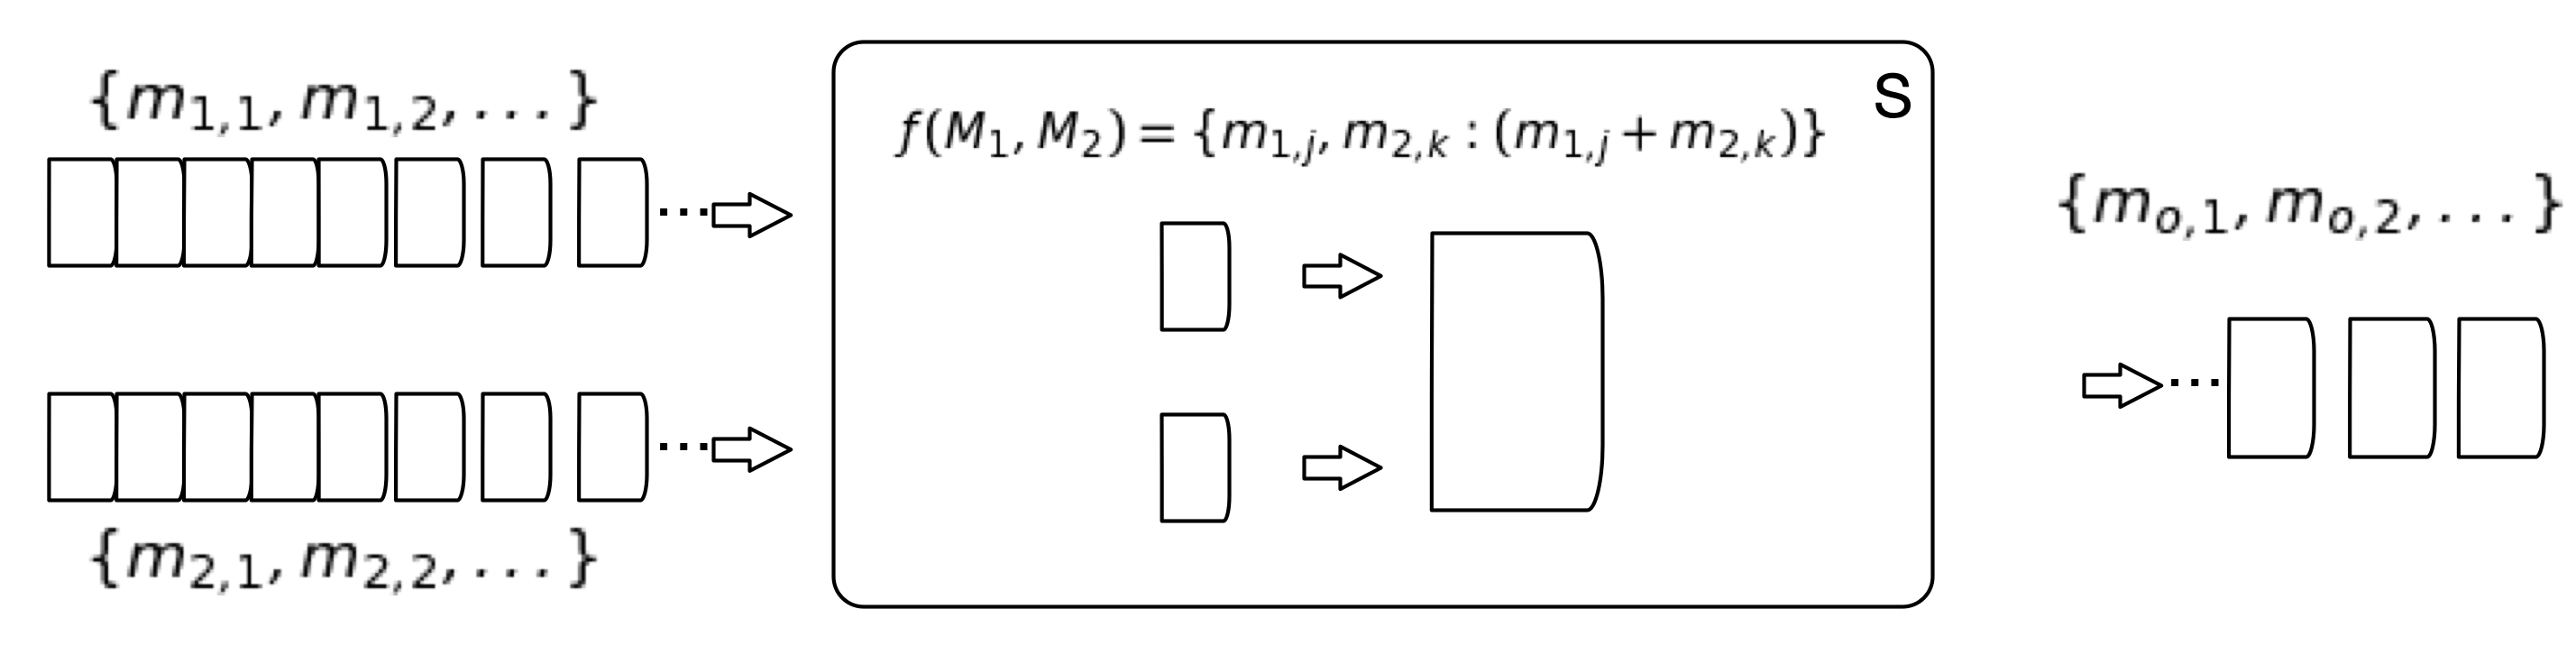
\includegraphics[scale=0.6]{stream_aggregator_function}
\centering
\caption {Service S integrates messages from multiple input streams $M_i$ to produce an aggregated output stream $M_o$ via $f$.}
\label{fig:stream_aggregator_function}
\end{figure}


\paragraph{Local State Aggregator Function} - Service $S$ observes an input stream $M_i$ which it integrates with a local (non-stream) queryable data store (see Figure \ref{fig:stream_local_state_aggregator_function}). Messages $m_i$ are integrated with query results $q_i$ to produce an output stream $M_i$. This type of service also requires management of state and scalability concerns similar to the Aggregator service, especially when the local data store is itself distributed. 

\begin{figure}[H]
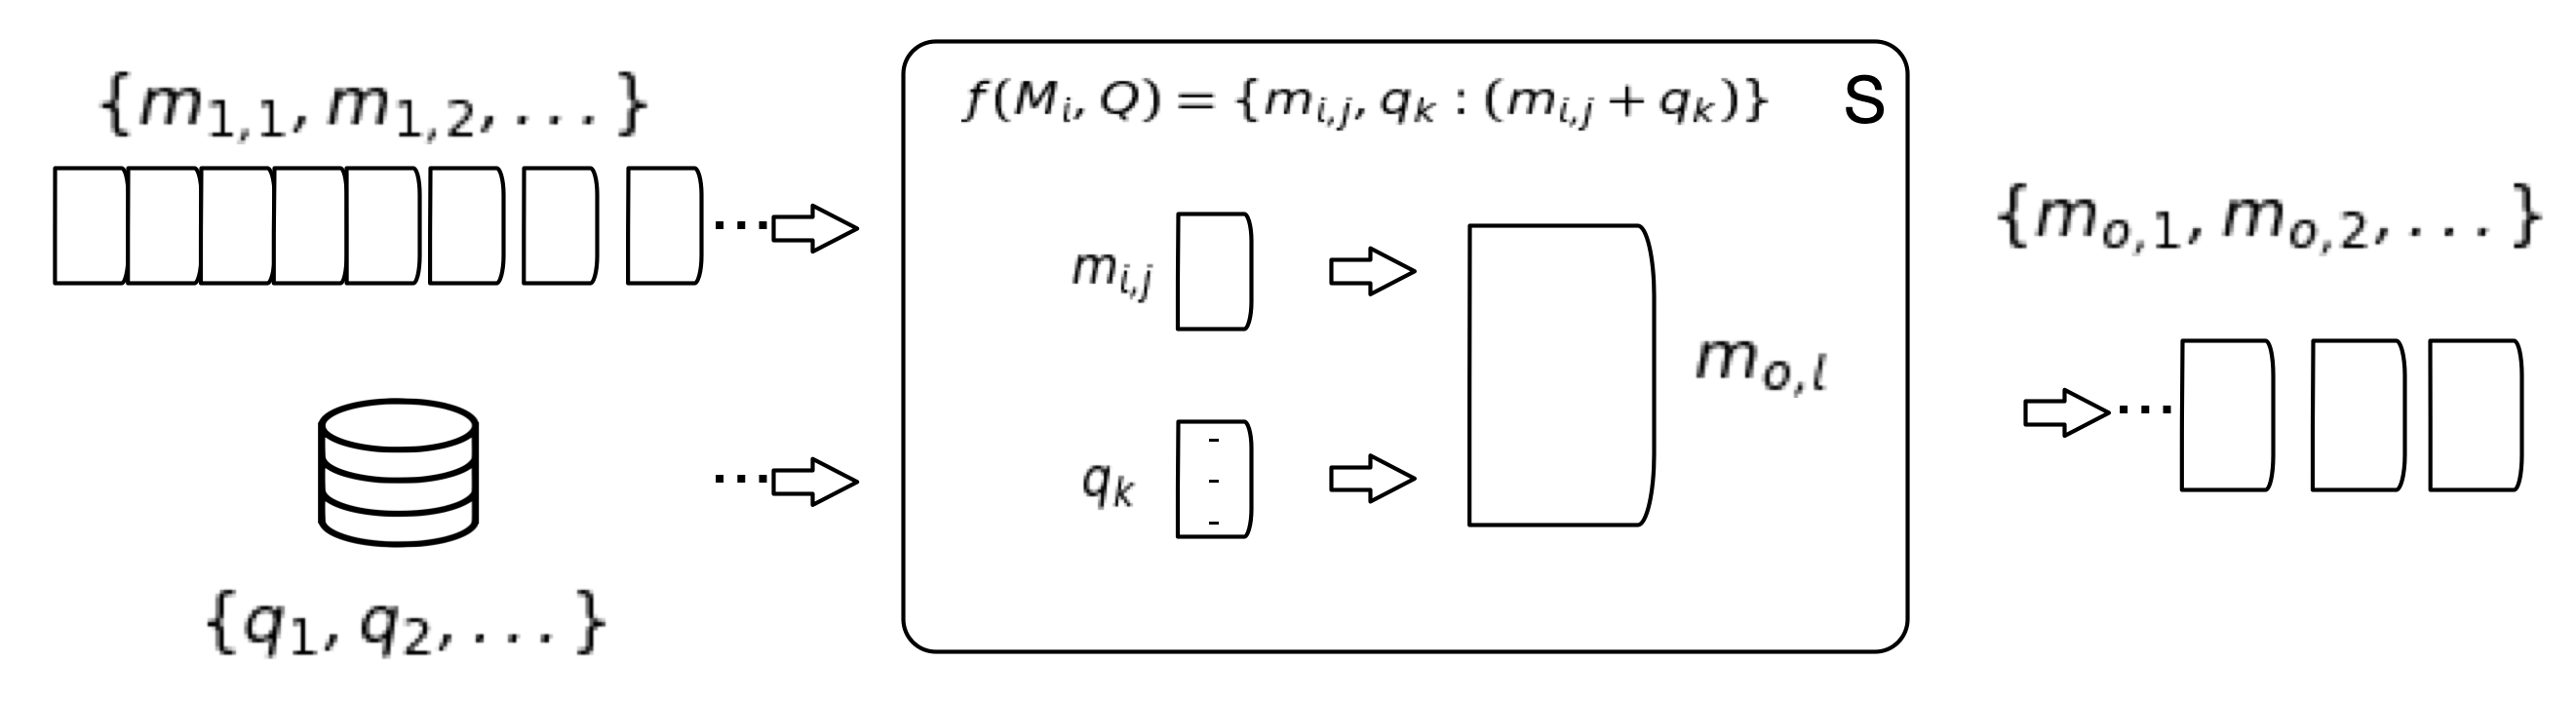
\includegraphics[scale=0.6]{stream_local_state_aggregator_function}
\centering
\caption {Service S aggregates $m_i$ with query results $q_i$ obtained from a local data store.}
\label{fig:stream_local_state_aggregator_function}
\end{figure}


\paragraph{Persistence Function} - Service $S$ observes messages $m_i$ and is responsible for persisting them to a data store where their contents can later be queried (see Figure \ref{fig:stream_persistence_function}). Although persistence of data to, and subsequent querying of data from, a store, such as a database, are comparatively more expensive operations than immediate reasoning over a live data stream, such mechanisms are necessary for situations where data may need to be accessed multiple times, or where data may need to be retained for audit purposes.

\begin{figure}[H]
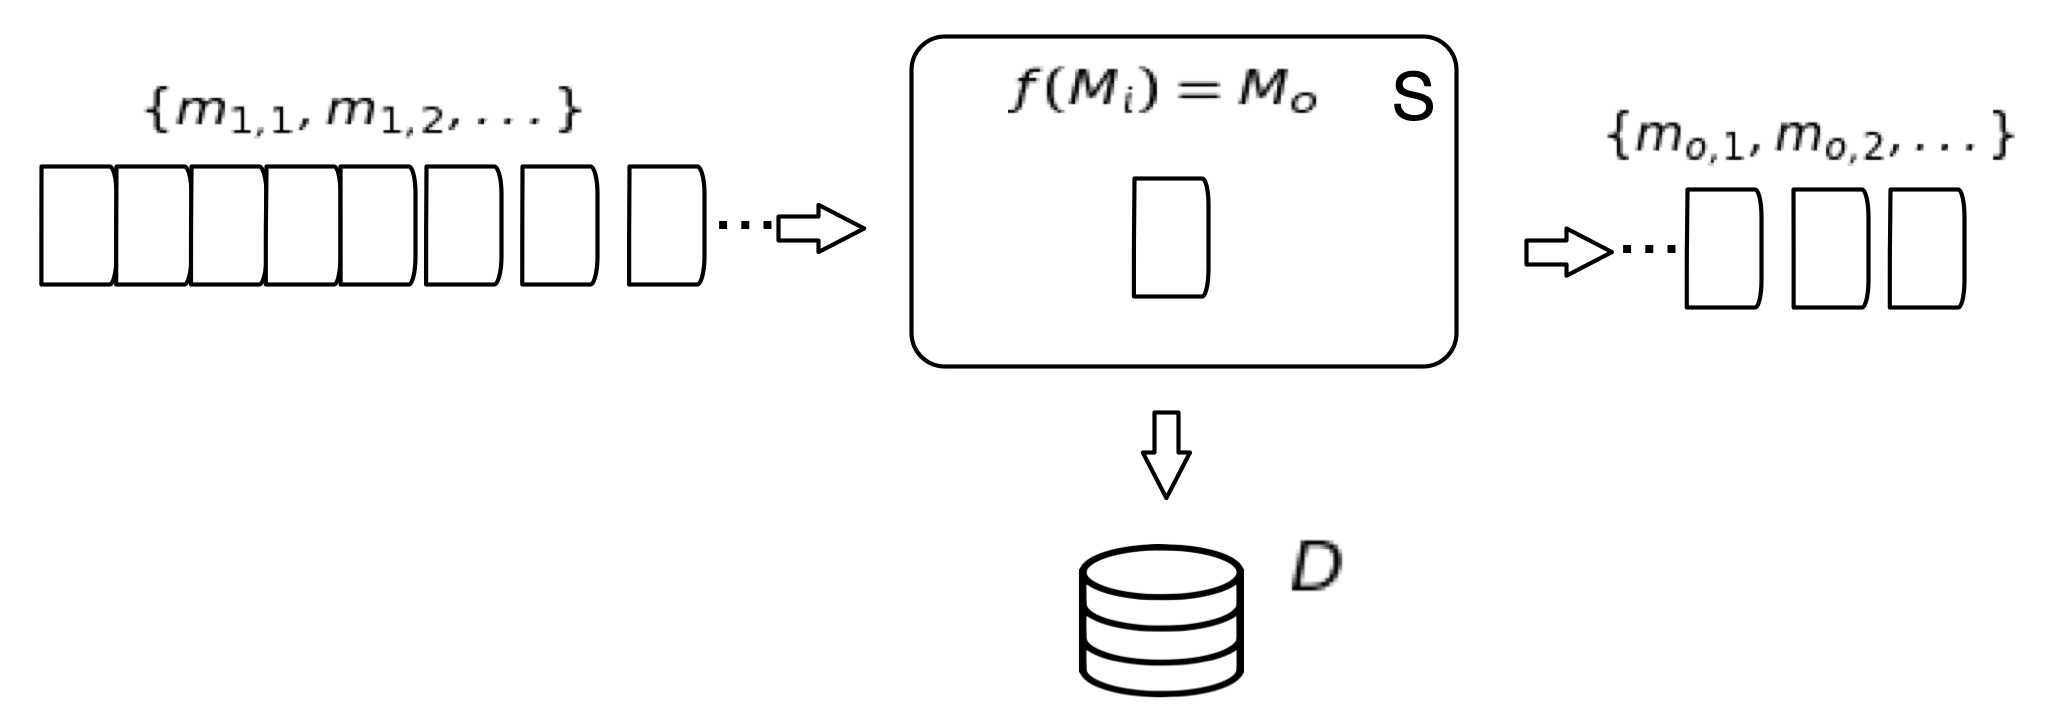
\includegraphics[scale=0.6]{stream_persistence_function}
\centering
\caption {Service $S$ processes messages $m_i$ into persistent storage. The output stream $M_o$ contains persistence confirmation and error events.}
\label{fig:stream_persistence_function}
\end{figure}

\paragraph{Query Function} - Service $S$ observes a stream of queries $Q_i$. The queries are fulfilled against a data store $D$ and the results emitted via the output stream $M_o$.

\begin{figure}[H]
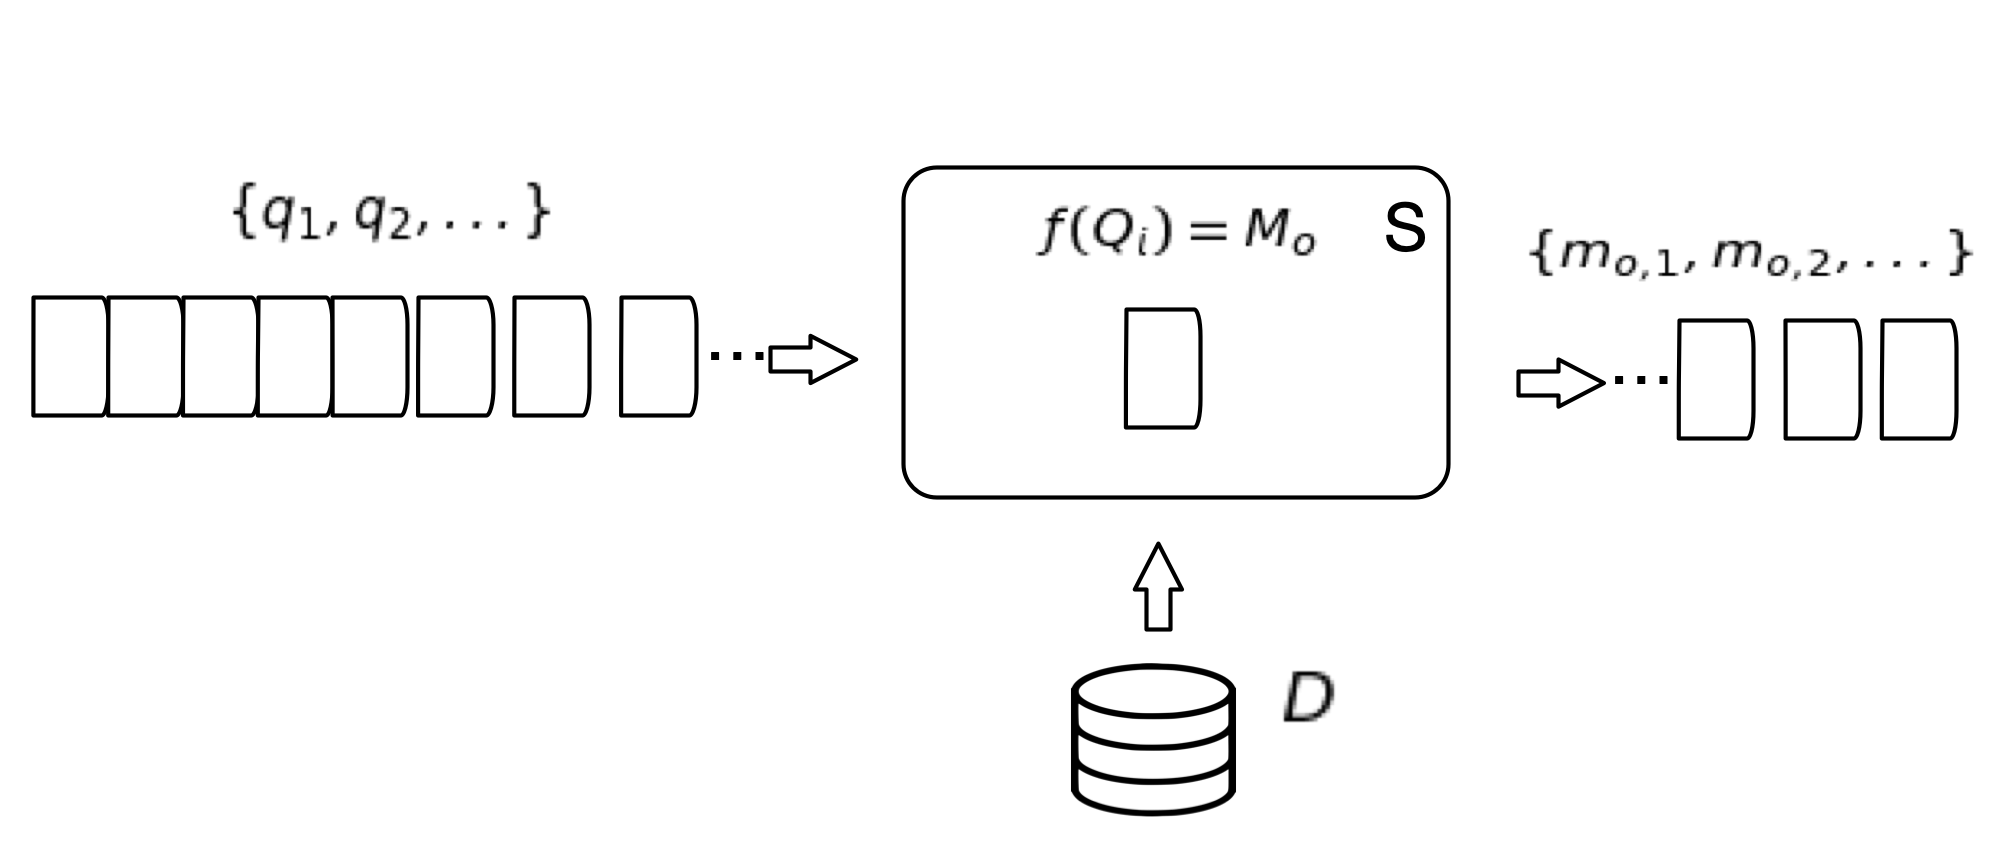
\includegraphics[scale=0.6]{stream_query_function}
\centering
\caption {Service S filters messages from input stream $M$ and only allows through those that pass the filtering condition.}
\label{fig:stream_query_function}
\end{figure}

The basic operations above can be combined to produce arbitrarily complex logic on data streams.

One of the key advantages of a service-oriented approach is that, because services are typically constantly executing, it naturally lends itself to an examination of the system's runtime characteristics. This applies to both service-internal characteristics that are related to each operation a service performs, as well as to external characteristics that relate to the contracts a service establishes with its dependencies. We consider both of these.

For each given operation $o_i \in S$ it is instrumental to understand the resource requirements of the operation on typical inputs and limiting factors that affect the efficiency with which the operation can be performed by $S$. Of particular interest are the per-operation profiles of:

\begin{itemize}
    \item CPU utilization
    \item RAM
    \item Secondary storage
    \item Network utilization
\end{itemize}

If $o_i$ is a long-running operation that takes multiple seconds to complete on average, a detailed distribution in time of each metric above may be necessary. If the operation can be completed at a sub-second rate then summary statistics (min, max, mean, median, inter-quartile range, 90th, and 99th percentiles) may be sufficient. This level of understanding is necessary in order to make sure that the service can adequately deal with the incoming message stream while the messages are first loaded into memory, since subsequent retrieval from secondary storage is several orders of magnitude slower and may cause further delays in processing. If $o_i$ is stateless, i.e. it does not require the storage and retrieval of any local state that depends on the content of each arriving message $m_j \in M_i$, then the service $S$ can be scaled "horizontally"\autocite{vaquero2011dynamically} with respect to $o_i$. Given that the performance-limiting condition of $o_i$ is known (CPU, memory, etc.), the ability of $S$ to efficiently deal with fluctuations in the rate of incoming messages $M_i$ can be successfully achieved simply by adding and removing servers that execute $S$ (see Figure \ref{fig:horizontal_vs_vertical_scaling}), which can be done automatically\autocite{mao2011auto}. If $o_i$ is stateful and requires access to databases, or predictable request routing via sessions, then horizontal scalability may not be possible and thus, detailed understanding of the performance profile and performance-limiting conditions of $o_i$ is even more important as vertical scaling of services is more expensive and challenging to accomplish, and may increase system complexity by necessitating data partitioning, for example\autocite{vaquero2011dynamically}.

\begin{figure}[H]
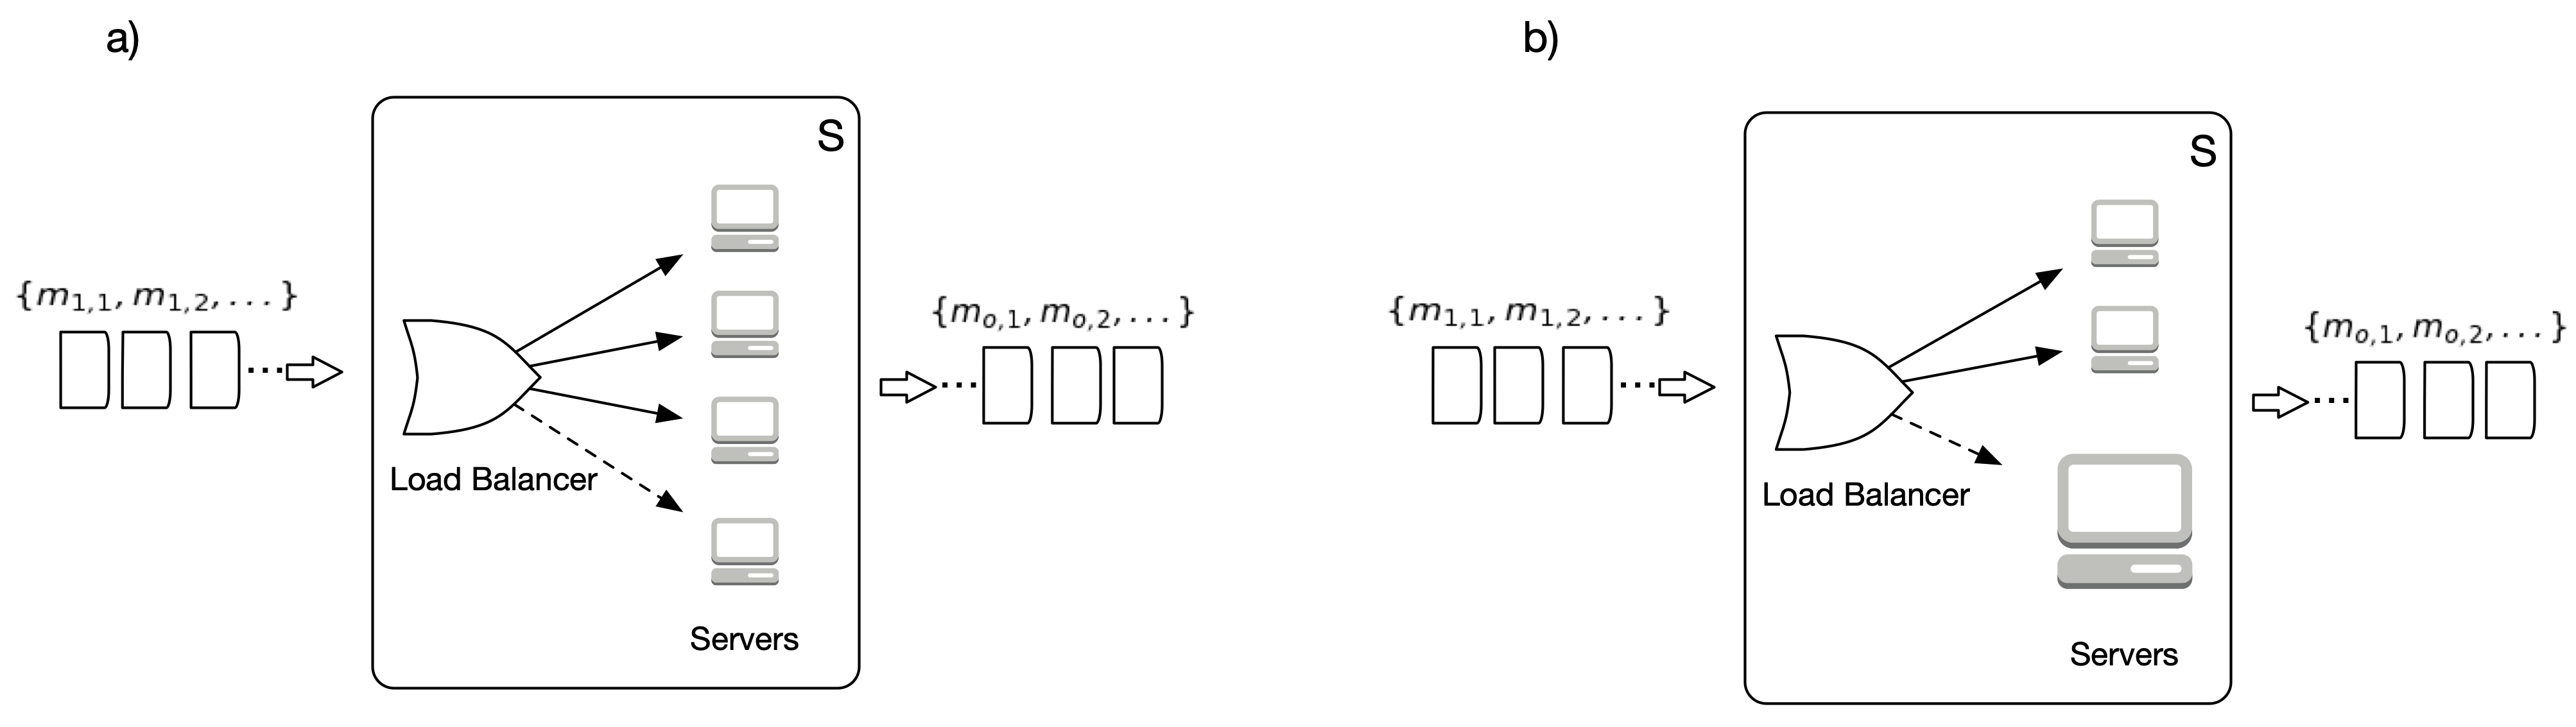
\includegraphics[scale=0.44]{horizontal_vs_vertical_scaling}
\centering
\caption {a) In horizontal scaling new servers are added and removed (dashed arrow) behind a load balancer as the rate of data stream $M_i$ fluctuates. b) In vertical scaling more powerful servers need to be launched (dashed arrow) to replace smaller servers (with potential service outage) when the rate of $M_i$ increases beyond capacity.}
\label{fig:horizontal_vs_vertical_scaling}
\end{figure}

Assume service $S$ implements operation $o$ supported by $n$ physical servers $V = \{v_j: j \in [1,n]\}$ by consuming a stream of incoming messages $M_i$. For a suitable time increment $t$, let $r_{M_i} = |M_i|/t$ be the incoming message arrival rate, and $r_{M_{o,j}} = |M_{o,j}|/t$ be the processing rate for server $v_j$. If $r_{M_i} > \sum_{j=1}^n r_{M_{o,j}}$, then $S$ will not be able to adequately process all of the incoming messages from $M_i$ and messages will either be lost or need to be backlogged while more servers are added to $S$ to deal with the incoming message rate. Since commissioning new servers takes considerable time and the timing and magnitude of increases in $r_{M_i}$ may be unpredictable, serious information loss may result if measures are not put in place to mitigate the message rate fluctuations. 

A queue is the mechanism that we put in place to address this concern (see Figure \ref{fig:queue}). A queue $Q$ is a message buffering system which consists of a set of $n$ "topics" $P = \{p_i: i \in [1,n]\}$, where each topic is a tuple of the form $p_i = (D_p,B_p,C_p)$. Here $D_p = \{d_i: i\in [1,k]\}$ is a set of $k$ data producers that put messages into $Q$, $B_p$ is a message buffer of max capacity $N_{max}$ dictated by underlying server hardware characteristics, containing a sequence of messages $\{m_t, m_{t-1},m_{t-2},....,m_1\}$ that are accessible in a Fist In First Out (FIFO) manner, and $C_p = \{c_i: i \in [1,l]\}$ is a set of $l$ consumers that are interested in observing messages from $p_i$.

\begin{figure}[H]
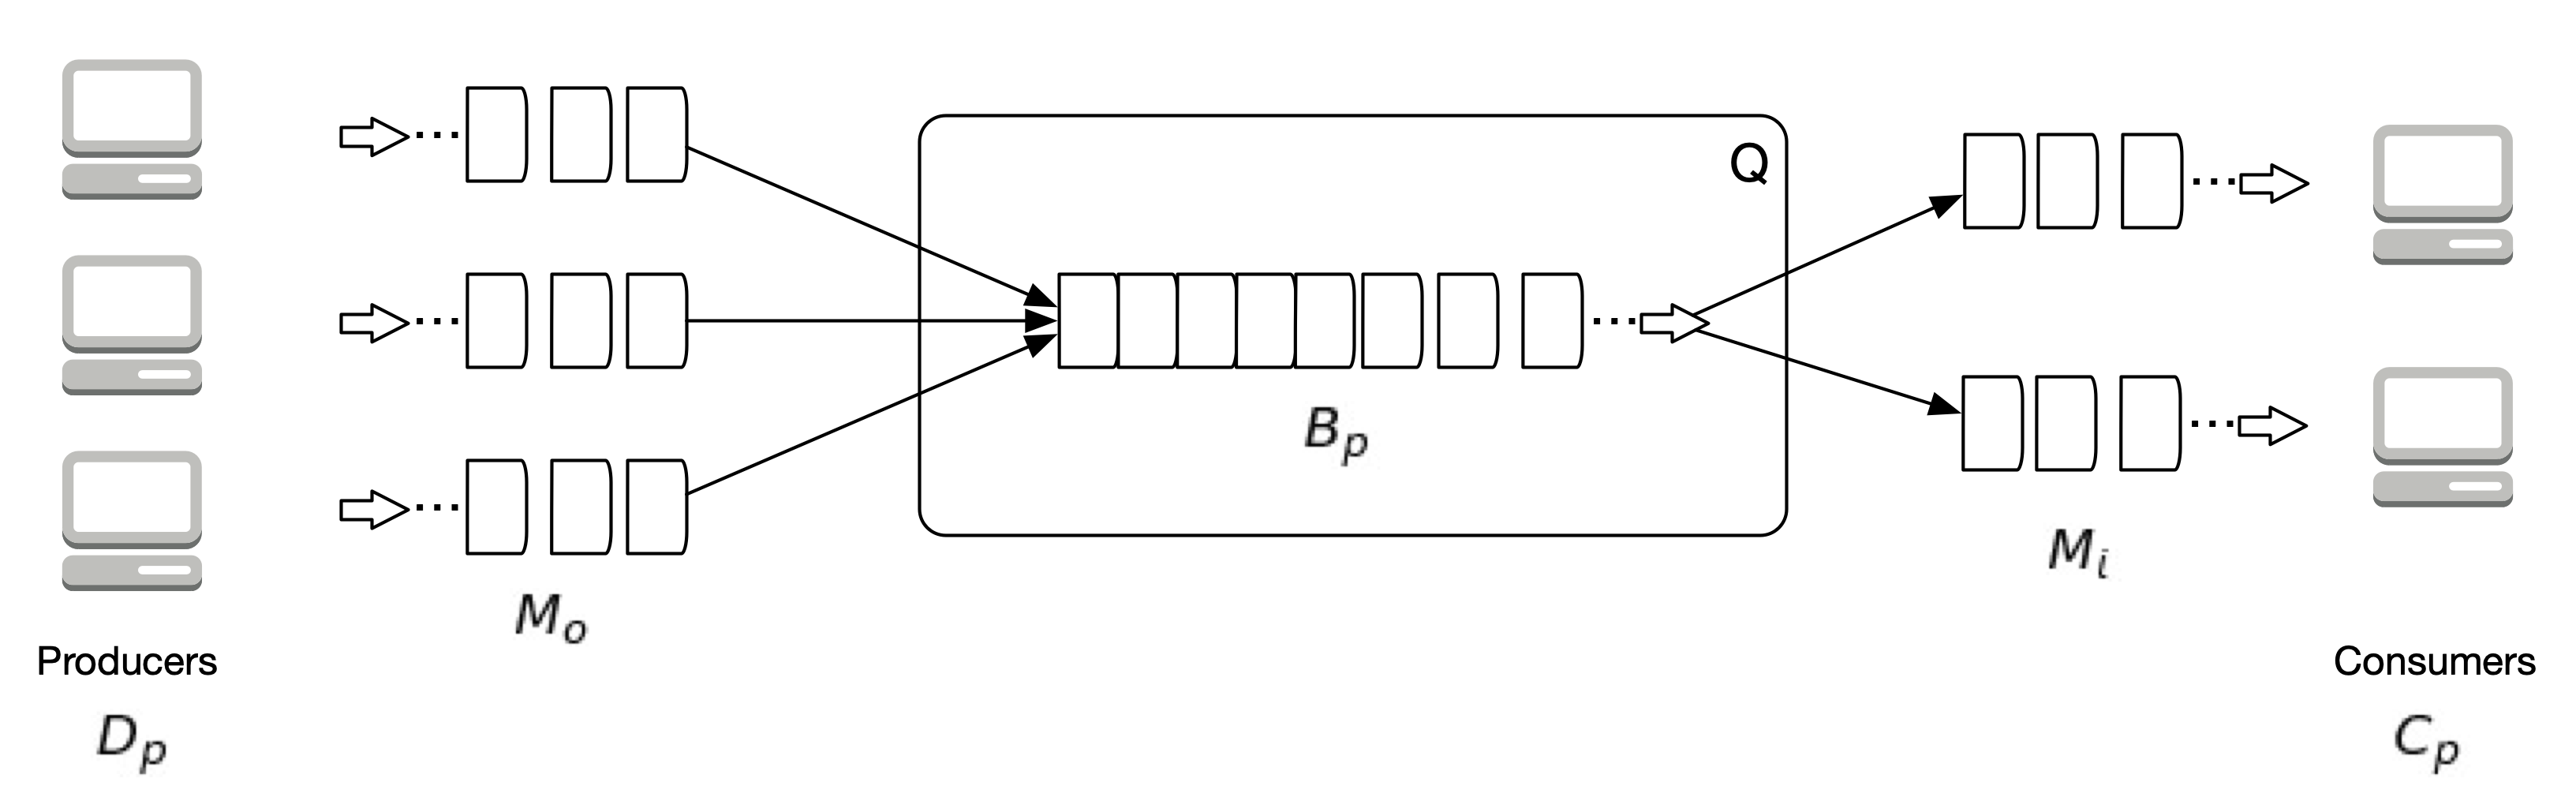
\includegraphics[scale=0.54]{queue}
\centering
\caption A queue $Q$ establishes a message buffer $B_p$ between a set of message producers $D_p$ and consumers $C_p$, for a given topic $p$.
\label{fig:queue}
\end{figure}

Messages arrive into a particular topic of $Q$ from all producers $D_p$, and are marked safe for deletion only when all of the subscribed consumers $C_p$ have observed a particular message. Thus, for topic $p_i$, the incoming message rate is $\displaystyle R_i = \sum_{j=1}^k r_{M_{o,j}}$ i.e. the sum of the message processing rates for all of the producers for this topic. The queue message processing rate $\displaystyle R_o = \min_{i \in [1,l]}\{r_{M_{o,i}}\}$ is the slowest message processing rate among all consumers. Assuming $R_i > R_o$ and that there are $N$ messages presently in $B_p$, there remains $t = \frac{N_{max} - N} {R_i - R_o}$ time before queue overflow occurs. The situation should then be remedied by allocating additional hardware to $Q$ or those services $S_i$ whose consumers are slowest, until the condition $R_o \ge R_i$ can be reliably maintained. If the queue does reach its maximum capacity overflow measures need to be put in place. Depending on the data stream in question data loss may or may not be acceptable. If data loss is acceptable then overflow messages can be simply discarded. If data loss is not acceptable then producers must block waiting for additional queue capacity to become available. This not only degrades performance locally, but can have a drastic effect on the entire system if the effects are allowed to percolate trough the complex distributed system. As message rates evolve through time with system load, the scheme above sets up a framework for flow control and hardware allocation within the architecture.

When designing a service-oriented system the interfaces of operations provided by the service are of utmost importance as they define the capabilities that the service offers to its clients. Of secondary, but also significant, importance is the set of Service-Level Agreements (SLAs)\autocite{wieder2011service} that a service advertises. These SLAs are a set of commitments that a service makes to its clients that describe the operational characteristics of the service, such as:

\begin{description}
    \item [Availability] - Guarantees related to the service uptime, maintenance outages, disaster recovery, etc.
    \item [Throughput] - The number of requests serviced per unit time.
    \item [Latency] - The delay between a request being sent and a response being received.
    \item [Abandonment Rate] - Proportion of requests that are never answered.
    \item [Error Rate] - Proportion of well-formed requests that result in an error.
\end{description}

Based on the SLAs that are advertised by a given service, the services that depend on it can make assumptions about expected runtime behavior, and take action when expectations are not met. Furthermore, when requirements evolve and features are added to or removed from a service, the impact on the advertised SLAs helps communicate the full effect of the changes. Lastly, the costs of operating a service are more clearly understood through the SLA framework, where improvements to a particular SLA metric, such as Transactions-Per-Minute (TPM) can be transparently traced to a corresponding increase in operational costs.

The set of services $\{S\}$ that communicate over data streams $\{M_{s,d}\}$, mediated by a set of queues $\{Q\}$ with a set of established SLAs $\{L_s\}$ together form the overall framework of Rheos that is used to tackle the challenges of large-scale genomic data processing in a manner the enables active tradeoffs between the competing constraints of cost, time, and accuracy. 

\section{Domain-specific Problems}

Having laid out the general data-streaming service-oriented architecture of Rheos in the previous section we now turn to a discussion of the set of actual domain-specific problems that need to be solved within the data-streaming paradigm in order to enable the comprehensive genomic characterization of large cohorts of samples within Rheos, as we have set out to do. We make use of the flow of data types from the most raw to the most refined (see Figure \ref{fig:ngs_flow}) to illustrate the challenges that need to be solved during transformation of the input data between each successive stage, first in summary form, and then in full detail, below.

\begin{figure}[H]
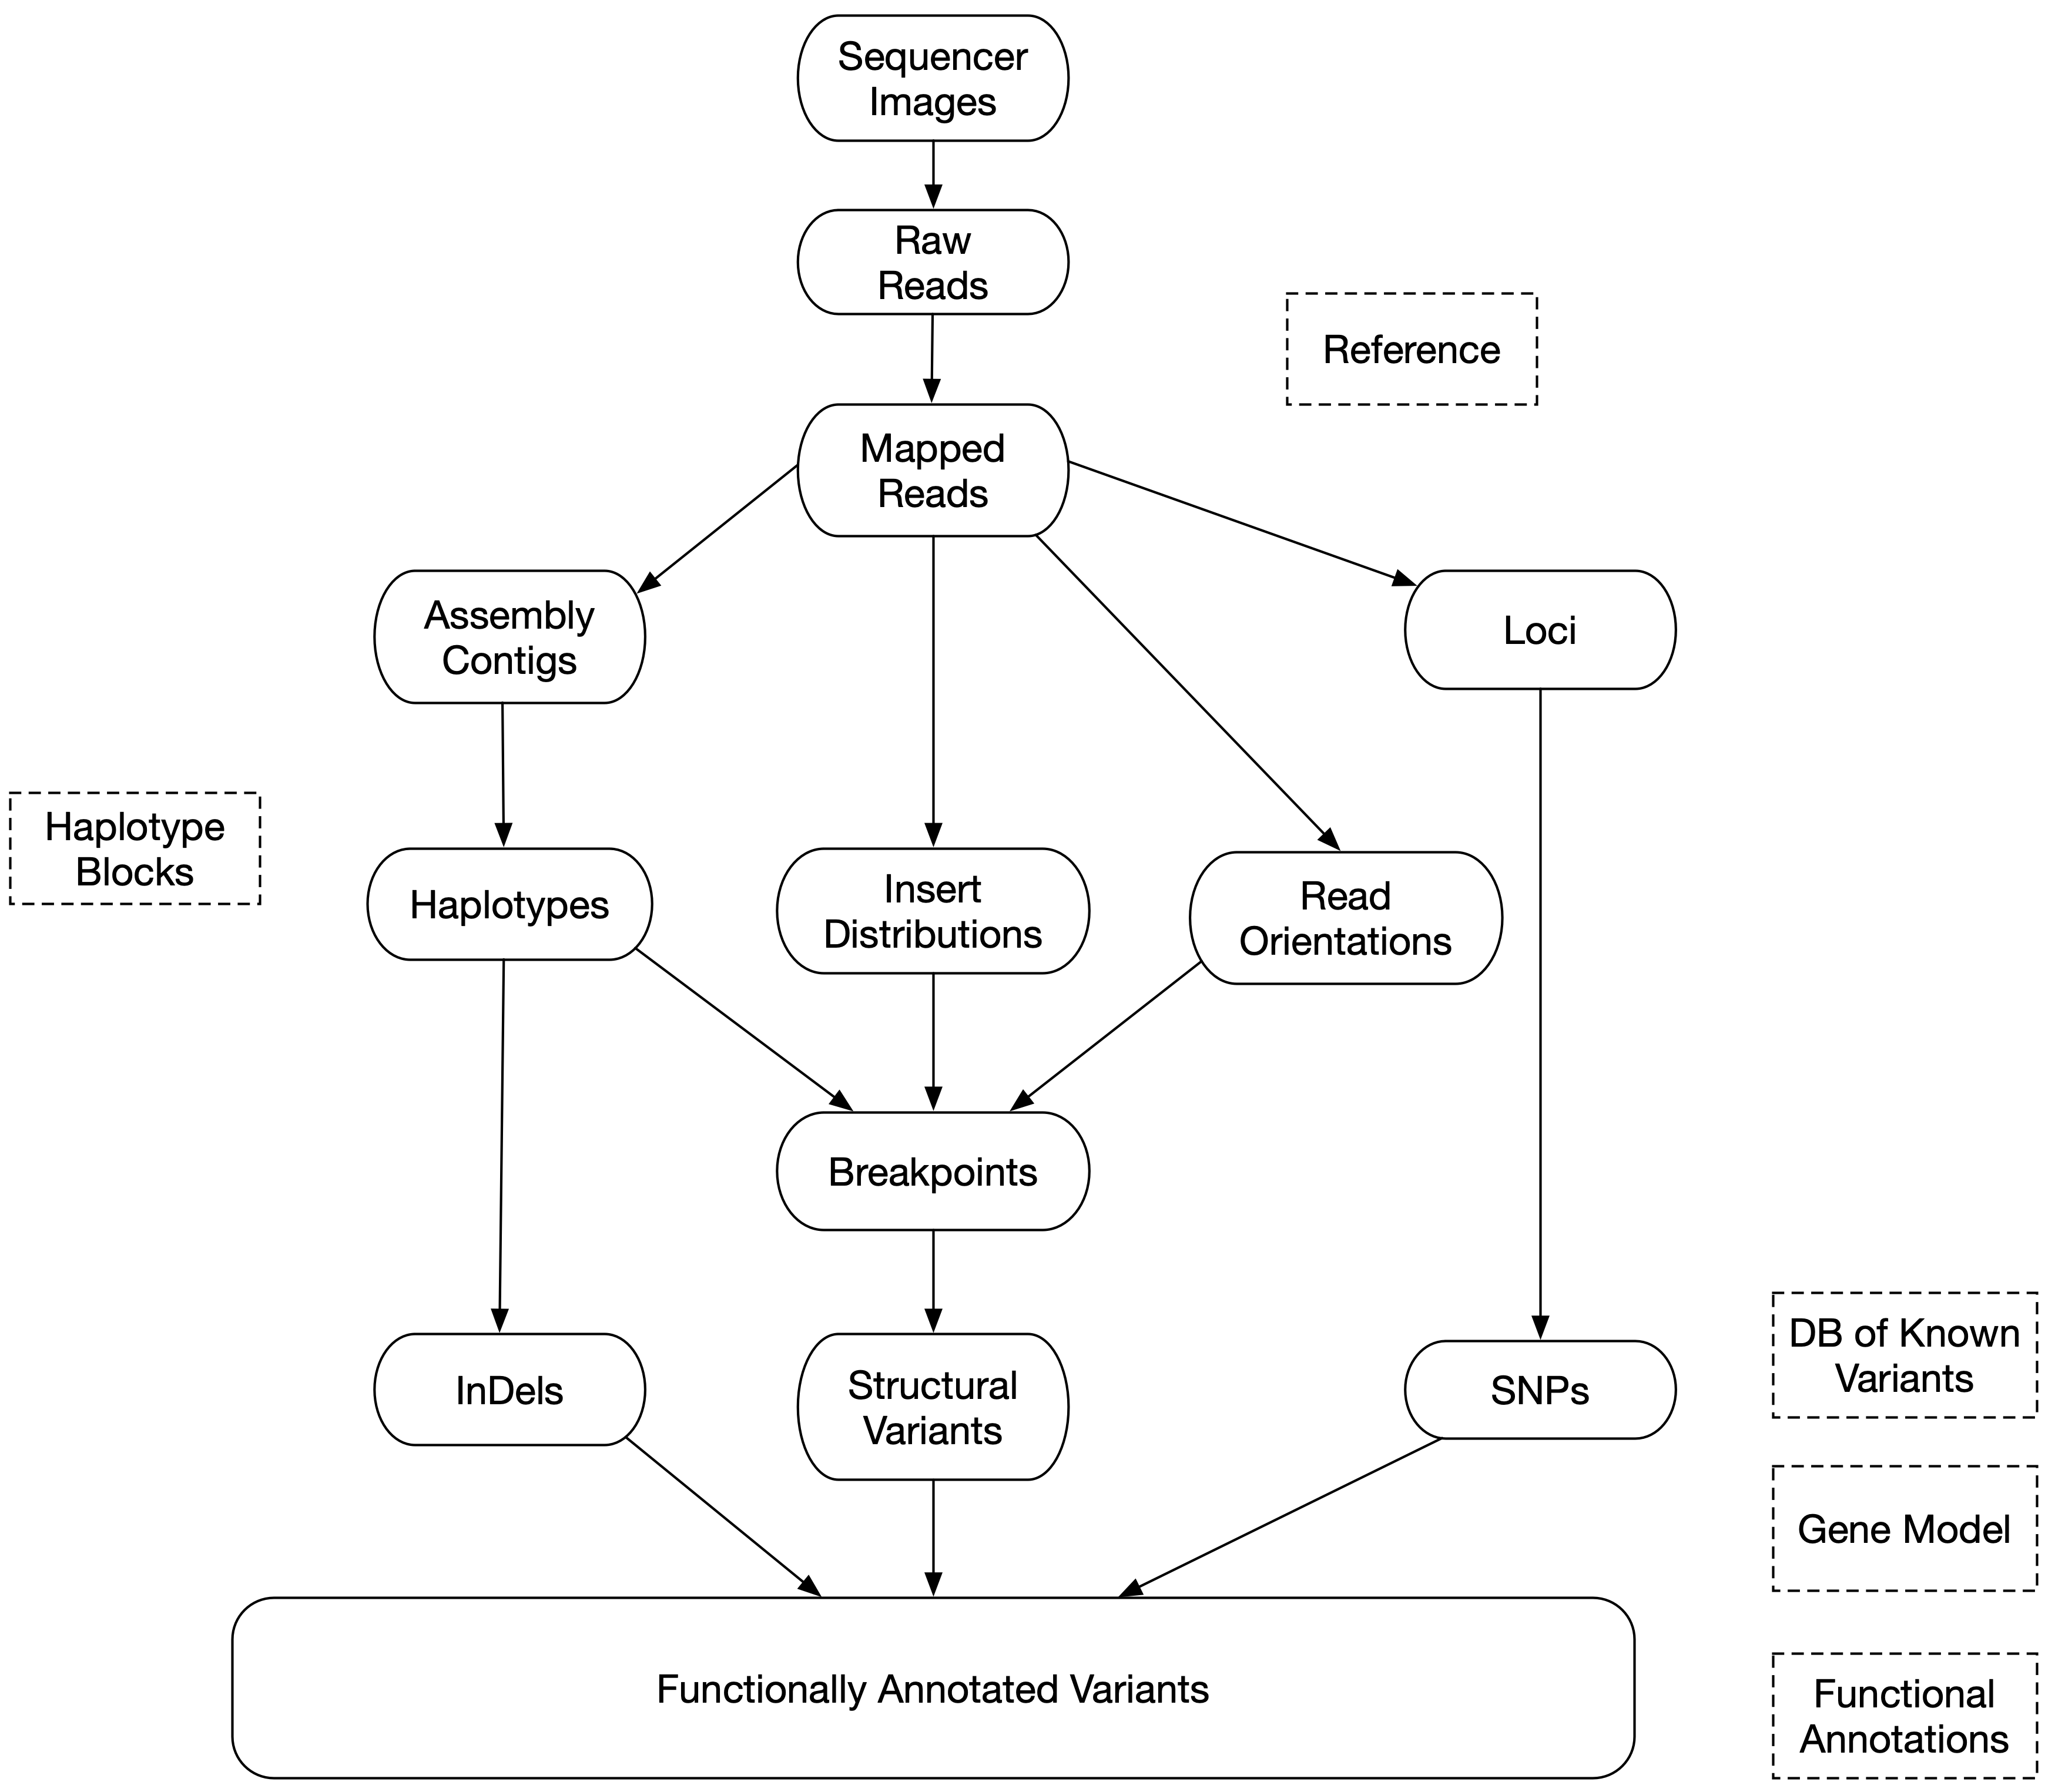
\includegraphics[scale=0.5]{ngs_flow}
\centering
\caption {The conceptual flow of data types within Rheos from the most raw - Sequencer Images, to the most refined - a set of Functionally Annotated Variants.}
\label{fig:ngs_flow}
\end{figure}
    
The most raw data type that is produced from a sequencing experiment is the set of raw image files generated by the sequencer. Although, conceptually, processing of the raw images could also be accomplished within Rheos, it is presently outside of the scope of this work. Instead, we assume the most basic data type to be raw sequencing reads, as found in a FASTQ\autocite{cock2009sanger} file. 

\begin{figure}[H]
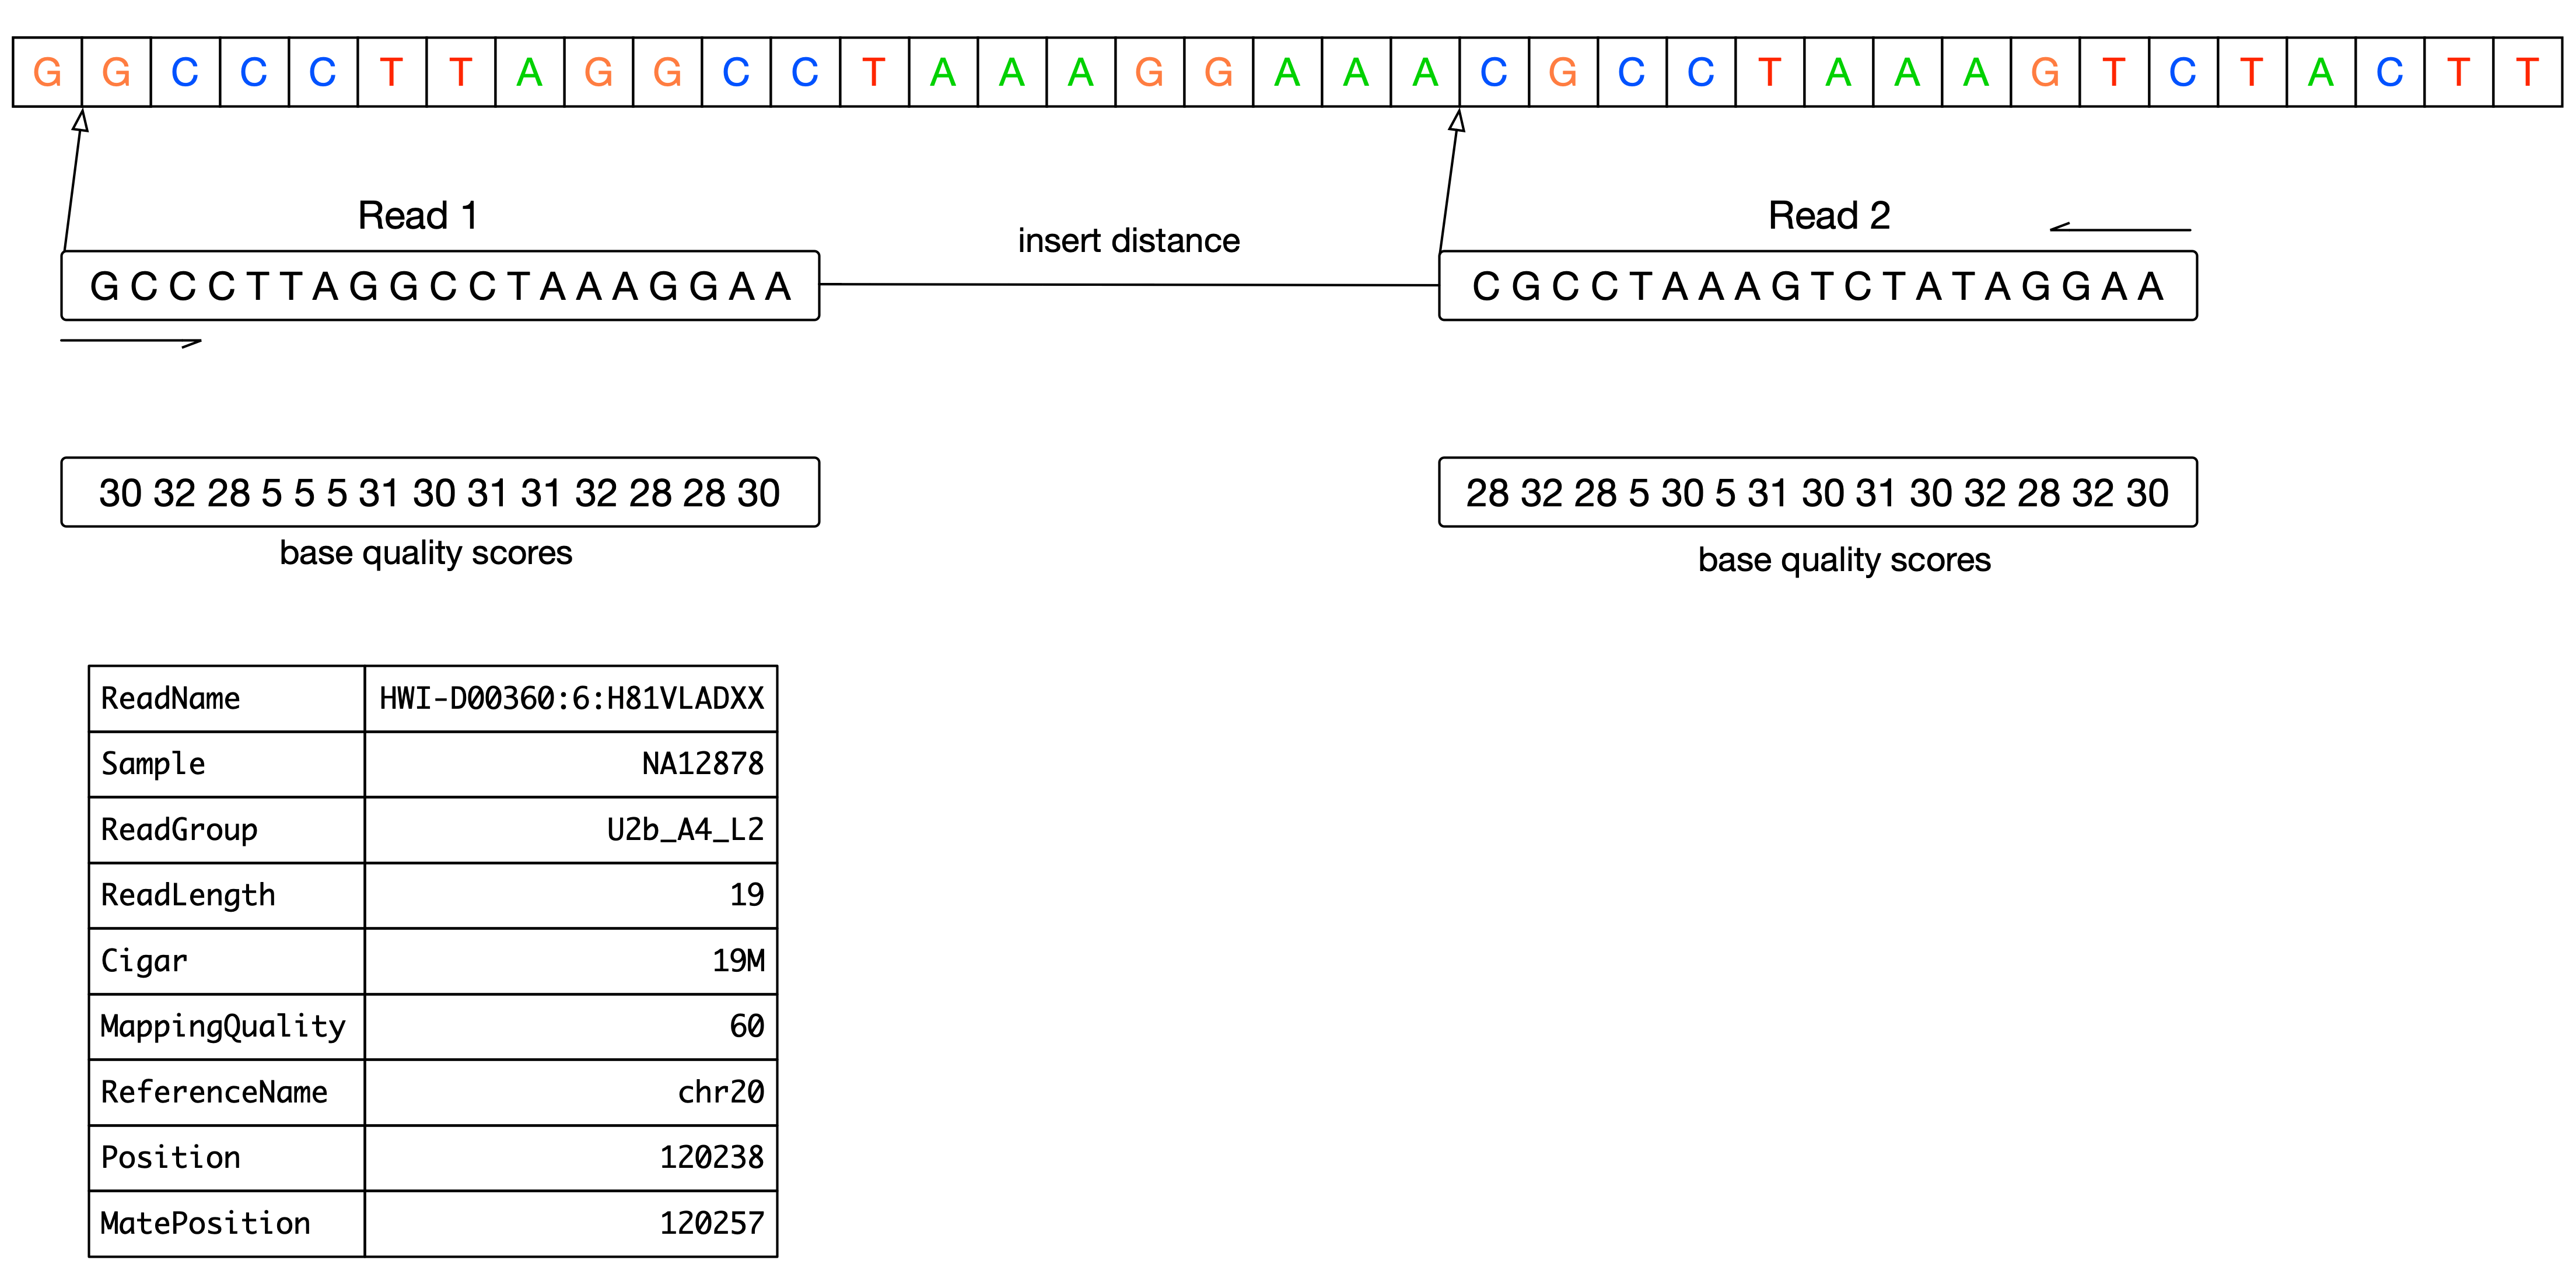
\includegraphics[scale=0.40]{read_pair}
\centering
\caption {A read-pair that is aligned to the reference.}
\label{fig:rheos_read_pair}
\end{figure}

Each read is a tuple of the form:

\begin{equation}
\label{eq:raw_read_message}
r = (s\_id, r\_id, b, q, f_p)
\end{equation}

where:

\begin{itemize}
    \item $s\_id$ - is the sample ID, which is unique among all samples.
    \item $r\_id$ - is the read ID, which is unique among all reads for that sample.
    \item $b = \{b_1, b_2,.....,b_n\}$ - is the sequence of DNA bases, where $b_i \in \{A,C,G,T,N\}$.
    \item $q = \{q_1, q_2,....,q_n\}$ - is the set of PHRED-scaled base quality scores corresponding to the probability that the base has been called incorrectly. See discussion on FASTQ format in Section \ref{sec:bg_file_formats} for details.
    \item $f_p \in \{True, False\}$ - is a boolean flag indicating whether this read is the first read in a pair.
\end{itemize}

\subsection{Read QC Metrics}
\label{sec:main_body_read_qc_metrics}

Section \ref{sec:bg_raw_data_qc} of the Background chapter discusses various metrics of interest that are based on observations of read data and the tools that are used to collect them. Here we describe how to collect the most typical metrics in the streaming paradigm of Rheos. As before, there are per-read metrics such as Base Quality Distribution, and Adapter Sequence Presence, as well as per-sample metrics such as Average GC Content, Insert Distribution, Read Length Distribution, and others. The utility of these metrics is to be able to set up filters for low quality data as well as input for downstream variant-calling models (see Section \ref{sec:bg_germline_sv_calling} for example). 

Assume that we are observing a stream $M_{raw} = \{m_i: m_i = (header, payload)\}$ of read messages where the payload is a read $r$ as defined above. Under the assumptions of Section \ref{sec:rheos_streaming_architecture} we know that the number of elements in the stream is unbounded. We are able to straightforwardly calculate incremental estimates for metrics such as mean, variance, max, and min, but require more sophisticated structures for computing estimates of rank statistics such as median and other quantiles to maintain operations in bounded space. We use the following update rules for min, max, mean, and variance\autocite{welford1962note} calculations:

\begin{equation}
    \label{eq:stream_min}
    min_k(M) =  \begin{cases}
        m_k,& \text{if } m_k < min_{k-1}(M)\\
        min_{k-1}(M),& \text{otherwise}
    \end{cases}
\end{equation}

\begin{equation}
    \label{eq:stream_max}
    max_k(M) =  \begin{cases}
        m_k,& \text{if } m_k > max_{k-1}(M)\\
        max_{k-1}(M),& \text{otherwise}
    \end{cases}
\end{equation}

\begin{equation}
    \label{eq:stream_mean}
    \mu_k(M) =  \mu_{k-1}(M) + \frac {m_k - \mu_{k-1}} {k} 
\end{equation}

\begin{equation}
    \label{eq:stream_variance}
    \sigma_k^2(M) =  \frac{\sigma_{k-1}^2(M) + (m_k - \mu_{k-1}(M))(m_k - \mu_k(M))}{k-1} 
\end{equation}

In order to set up the mechanisms to answer quantile queries the following definitions are used\autocite{garofalakis2016data}:

\begin{itemize}
    \item Given a set $S$ of size $n$, and a quantile $\phi \in [0,1]$, return $v \in S$ whose rank in sorted $S$ is $\phi n$. 
    \item An $\epsilon$-approximate $\phi$-quantile is a value $v$ whose rank $r*(v) \in [n(\phi-\epsilon), n(\phi+\epsilon)]$.
    \item A quantile summary is $Q = {q_1,q_2,....,q_l: q_1\le q_2 \le \dots \le q_l, q_i \in S, i \in [1,l]}$ where each $q_i$ has rank at least $rmin_Q(q_i)$ and at most $rmax_Q(q_i)$ in $S$, and $rmax_Q(q_1) \le \epsilon|S|$, and $rmin_Q(q_l) \ge (1-\epsilon)|S|$.
    \item A quantile summary $Q(\epsilon)$ is $\epsilon$-approximate if it can be used to answer any quantile query with $\epsilon$-accuracy.
\end{itemize}

We use two approaches for computing quantile summaries, one due to Greenwald and Khanna\autocite{greenwald2001space} is able to compute the quantile summary using $O(log(\epsilon n)/\epsilon)$ space, and the other by Shrivastava et al.\autocite{shrivastava2004medians} computes the quantile summary in $O(log(M)/\epsilon)$ when the values are integers in range $[1,M]$. Both algorithms work for a scenario where one node sees all of the data in a stream, but can also be generalized to topologies where the stream is observed by multiple nodes in parallel. 

We provide several examples of QC queries of interest that are specified on a data stream:

\paragraph{Average Base Quality} -  As an assessment of the individual quality of each read we are interested in the average base quality so that we can filter out reads that are of low quality as a whole. We use a Decorator Function construct from Section \ref{sec:rheos_data_streaming_model}. 

\bgroup
\def\arraystretch{1.5}
\begin{table}[!ht]
    \caption{Definition of $q_{av}$ which computes average base quality for a read}
    \label{tab:op_average_base_quality}
    {\begin{tabular}{l|p{12cm}}
    \toprule
    Inputs & \hangindent=1em$M_{raw} = \{m_i: m_i = (header, payload)\}$ where $m.payload = r = (s\_id, r\_id, b, q, f_p)$ as in \ref{eq:raw_read_message}.\\
    \cline{2-2}
    Operation & $q_{av} = \frac{\sum_{i \in [1,|r|]} r.q_i}{|r|}$\\
    \cline{2-2}
    {Outputs} & \hangindent=1em$M_{out} = \{m_i: m_i = (header, payload)\}$ where $m.payload = r = (s\_id, r\_id, b, q, f_p, q_{av})$\\
    \bottomrule
    \end{tabular}}
\end{table}
\egroup


\paragraph{Base Quality Distribution} - The distribution of base quality scores per base position of a read and per sample are of interest to investigate the presence of systemic biases in base quality scores as a function of the position within the read.

\begin{figure}[H]
    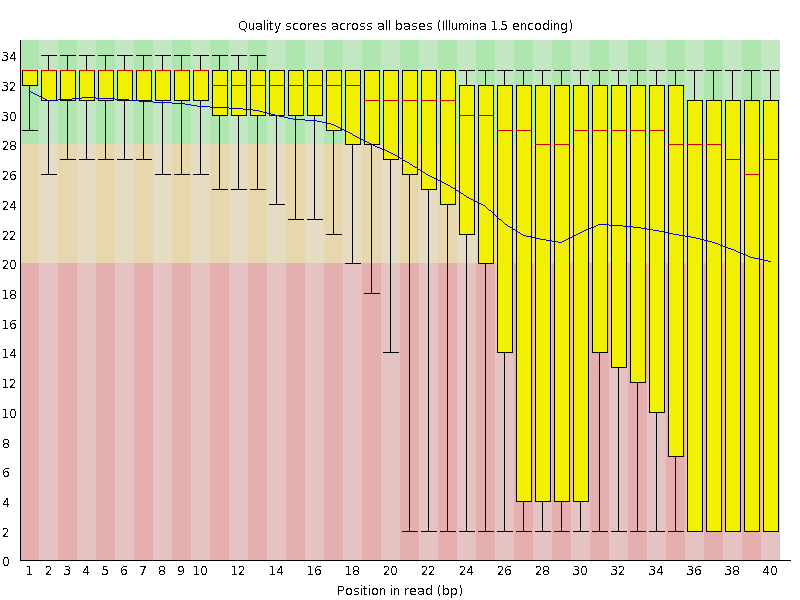
\includegraphics[scale=0.35]{fastqc_per_base_quality}
    \centering
    \caption {Distribution of base qualities per read position, from https://www.bioinformatics.babraham.ac.uk/projects/fastqc. Large quality drop-off can be see towards the end of the read.}
    \label{fig:main_body_fastqc_per_base_quality}
\end{figure} 


Because PHRED-scaled quality scores are integers that fall in a fixed range $q \in [0,96]$ building quantile summaries using the q-gram\autocite{shrivastava2004medians} approach is the most space-efficient. Because base quality scores need to be aggregated over many reads and tracked for many samples, a service that implements this functionality needs to keep local state, and the operation to update the quantile summaries based on incoming reads follows the Local State Aggregator pattern from Section \ref{sec:rheos_data_streaming_model}. 

\bgroup
\def\arraystretch{1.5}
\begin{table}[!ht]
    \caption{Definition of $updateQuantileSummaries()$}
    \label{tab:op_update_quantile_summaries}
    {\begin{tabular}{l|p{12cm}}
    \toprule
    Inputs & \hangindent=1em$M_{raw} = \{m_i: m_i = (header, payload)\}$ where $m.payload = r = (s\_id, r\_id, b, q, f_p)$ as in \ref{eq:raw_read_message}. \\
    \cline{2-2}
    Operation & $updateQuantileSummaries(r)$\\
    \cline{2-2}
    {Outputs} & \hangindent=1em$M_{out} = \{m_i: m_i = (header, payload)\}$ where $m.payload = (s\_id, Q_{bqd})$.\\
    \bottomrule
    \end{tabular}}
\end{table}
\egroup

Since the local state required for storing the quantile summaries may not fit in memory and may need to be persisted to disk, updating the summaries may be too expensive to do for every single read that is observed in a read input stream. Instead, reads may be buffered into a set of reservoirs, triggering an update of the quantile summaries when the reservoir is full. The contents of the reservoir would then be purged and an updated set of quantile summaries $Q_s,{bqg} = \{q_i: i\in [1,max\_bases]\}$, where each $q_i$ is a quantile summary corresponding to the Base Quality Distribution at a particular read position, issued to the output stream (see Algorithm \ref{ag:update_quantile_summaries_bqd}).

\begin{algorithm2e}[h]
\DontPrintSemicolon
\footnotesize
    \textbf{Function} {\sc updateBQDQuantileSummaries}$(r)$
    \Begin {
        $reservoir \gets ${\sc getReservoir$(r.s\_id)$}\;
        $reservoir.${\sc addNewRead$(r)$}\;
        \If {$reservoir.isFull$}{
            $summaries \gets ${\sc getQuantileSummaries$(r.s\_id)$}\;
            \For{$read$ {\bf in} $reservoir$}{
                \For{$index,read.q$ {\bf in} $read$}{
                    {\sc updateQGram$(summaries[index], read.q)$} \tcp*{per \autocite{shrivastava2004medians}}\;
                }
            }
            {\sc purgeReservoir$(reservoir)$}\;
            {\sc outputQuantileSummary$(r.s\_id, summaries)$}\;
        }
    } 
\caption{Updating quantile summaries for Base Quality Distribution.}
\label{ag:update_quantile_summaries_bqd}
\end{algorithm2e}

\paragraph{Insert Size Distribution} - The insert size distribution is an important metric because it is not only indicative of the overall quality of a sample's data, but it is also used by structural variant calling to find read-pairs that map abnormally far apart (indicating a deletion), or abnormally close together (indicating an insertion). 

\begin{figure}[H]
    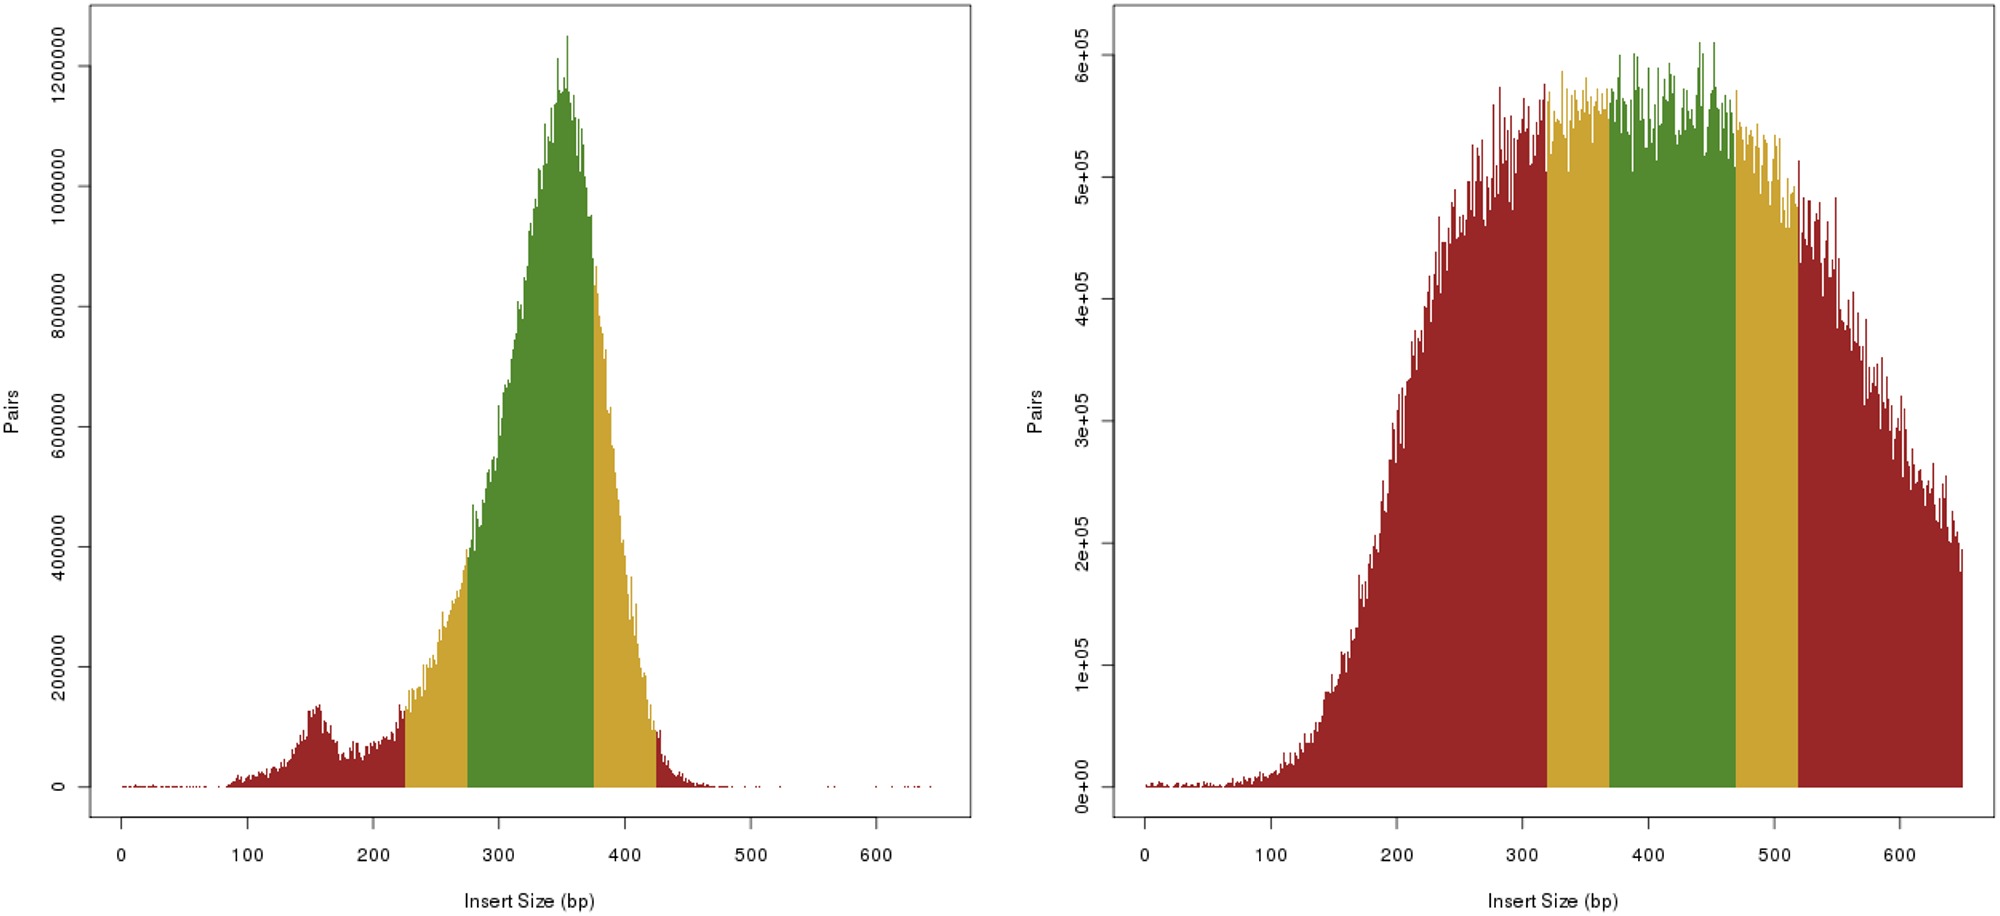
\includegraphics[scale=0.85]{insert_size_distribution}
    \centering
    \caption {Distribution of insert sizes from two ICGC pancreatic cancer patients DO35138 and DO22154.\autocite{stephens2016simulating}}
    \label{fig:insert_size_distribution}
\end{figure} 

Calculating this metric requires a stream of read-pairs, where both reads have been successfully mapped to the reference genome. Given a mapped read-pair $(r_1,r_2)$ where each read has a beginning coordinate $r.pos$ and an end coordinate $r.end$, the insert size is $l = r_2.end - r_1.pos$. We are interested in the mean, variance and quantiles of the insert size distribution. Because the insert length can be any size the quantile summary method of Greenwald and Khanna\autocite{greenwald2001space} is most appropriate for the quantiles. Read pairs are observed on the input stream and buffered in per-sample reservoirs. When a reservoir is full the read pairs are used to update and output an appropriate insert size distribution mean, variance, and quantile summary.

\bgroup
\def\arraystretch{1.5}
\begin{table}[!ht]
    \caption{Definition of $updateInsertSizeDistribution()$}
    \label{tab:op_update_insert_size_dist}
    {\begin{tabular}{l|p{12cm}}
    \toprule
    Inputs & \hangindent=1em$M_{pair} = \{m_i: m_i = (header, payload)\}$ where $m.payload = (r_1,r_2)$, and $r = (s\_id, r\_id, b, q, f_p)$ as in \ref{eq:raw_read_message}. \\
    \cline{2-2}
    Operation & $updateInsertSizeDistribution(s\_id,r_1, r_2)$\\
    \cline{2-2}
    {Outputs} & \hangindent=1em$M_{out} = \{m_i: m_i = (header, payload)\}$ where $m.payload = (s\_id, \mu_{isd}, \sigma_{isd}^2, Q_{isd})$.\\
    \bottomrule
    \end{tabular}}
\end{table}
\egroup

\begin{algorithm2e}[h]
    \DontPrintSemicolon
    \footnotesize
    \textbf{Function} {\sc updateInsertSizeDistribution}$(s\_id, r_1,r_2)$
    \Begin {
        $pairReservoir \gets ${\sc getReservoir$(s\_id)$}\;
        $pairReservoir.${\sc addNewReadPair$(r_1, r_2)$}\;
        \If {$pairReservoir.isFull$}{
            $summary \gets ${\sc getQuantileSummary$(s\_id)$}\;
            $mu \gets ${\sc getMu$(s\_id)$}\;
            $sigmaSq \gets ${\sc getSigmaSq$(s\_id)$}\;
            \For{($r_1, r_2$) {\bf in }$pairReservoir$}{
                $insertSize$ \gets $r_2.end - r_1.pos$\;
                {\sc updateQuantileSummary$(summary, insertSize)$} \tcc*{per \autocite{greenwald2001space}}\;
                $newMu$ \gets {\sc updateMu$(mu, insertSize)$} \tcc*{using Eq. \ref{eq:stream_mean}}\;
                $newSigmaSq$ \gets {\sc updateSigmaSQ$(sigmaSq, mu, newMu, insertSize)$} \tcc*{using Eq. \ref{eq:stream_variance}}\;
            }
            {\sc purgeReservoir$(pairReservoir)$}\;
            {\sc outputInsertSizeDistribution$(s\_id, newMu, newSigmaSq, summary)$}\;
        }
    }
    \caption{Updating metrics for Insert Size Distribution.}\label{ag:update_metrics_isd}
\end{algorithm2e}

Other QC metrics, such as those measuring GC Content Distribution, Read Length Distribution, etc. can be collected analogously. 

\subsection{Alignment}

Section \ref{sec:bg_alignment} of Chapter \ref{ch:background} provides an overview of the existing approaches in the extremely important and computationally intensive genome alignment stage of the overall NGS processing pipeline. In the overall data flow diagram (Figure \ref{fig:ngs_flow}), alignment is primarily responsible for transforming Raw Reads into Mapped Reads, but is also used in QC (insert size distribution, sample contamination) as well as in the construction and evaluation of local haplotypes for variant calling. In this section we describe the adaptation of already established read mapping best practices to the stream and services based domain of Rheos. Because of the generally independent nature of individual read observations (except for read pairs), this read mapping problem is highly amenable to a stream-based approach. We begin by enumerating and describing the types of alignment tasks that the Rheos framework needs to be able to accomplish and follow up by describing how these tasks will be performed within Rheos.

\begin{description}
    \item [Single read alignment to reference] - Given a representation of the human reference genome we are interested in finding a coordinate relative to this reference where the given read best matches. If we are not able to find a high quality mapping the read should be flagged as unmapped.
    \item [Read pair alignment to reference] - Given a pair of reads and an estimate of fragment size, attempt to find a high quality consistent mapping for both reads in a window around the expected fragment size.
    \item [Single read alignment to multiple references] - Given a read and a database of several genome references from multiple species determine if the read has a high quality mapping in any of the references. This can be used for assessing sample contamination.
    \item [Candidate haplotype alignment to reference] - Given a candidate haplotype i.e. a contiguous (potentially long) sequence locally assembled from a set of reads, align the sequence to the reference genome to identify locations of potential variation.
    \item [Single read alignment to list of alternative haplotypes] - Given a read and a list of alternative haplotypes for a region align the read to all of the haplotypes in the list to determine which haplotype is best supported by the reads.
    \item [Single read split-alignment to reference] - Given a read that does not align well to a contiguous region of the reference, search for an alignment where individual pieces of the read might align to separate and possibly distant locations on the reference, suggesting that the read spans a region of structural variation.
\end{description}

\paragraph{Single read alignment to reference} - Assume we are observing a data stream of raw unmapped short (<500 bp) reads $M_{raw} = \{m_i: m_i = (header, payload)\}$ where $m.payload = r = (s\_id, r\_id, b, q, f_p)$ as in \ref{eq:raw_read_message}. Using an existing human reference genome, such as \emph{GRCh38}, we would like to align each read in $m.payload$ to produce two new output streams $M_{aln}$ and $M_{unaln}$, depending on alignment results. $M_{aln}$, will contain messages from $M_{raw}$ with additional attributes related to the alignment, as described in Section \ref{sec:bg_sam_bam}, replicating the information contained in a SAM alignment record (see Table \ref{tab:sam_file_body_mandatory_fields}). $M_{unaln}$ shall contain reads from $M_{raw}$ that failed to align to a reference sequence, with an additional flag $unmapped=true$.

For $M_{aln}$ the following values are computed:

\begin{description}
    \item [rname] - name of the reference contig read is aligned to.
    \item [pos] - 1-based position offset of the left end of the read alignment to the contig specified in qname.
    \item [mapq] - Phred-scaled mapping quality representing probability that the read is misaligned.
    \item [cigar] - CIGAR string (as in SAM specification Section \ref{sec:bg_sam_bam}).
    \item [flags] - a tuple of flags as specified in the FLAG field of a SAM record.
\end{description}

Given that BWT and FM-index based algorithms\autocite{langmead2012fast},\autocite{Li2013} have currently shown the best balanced performance characteristics on both simulated and real data (see Figures \ref{fig:bwa_mem_comparison}, \ref{fig:bowtie_2_performance}) and the fact that these algorithms are amenable to straightforward parallelization, as in \autocite{langmead2009searching} for example, we adopt this approach as well in Rheos. Using this approach we will be able to locate $k$ locations for potential matches of a seed $d_i$ of read sequence $r.q$ in $\mathcal{O}(|r.q.d_i| + k)$ time using a data structure that takes $\mathcal{O}(|R|)$ space for a reference genome $R$. The seeds will then be extended using a version of Smith-Waterman\autocite{smith1981comparison} dynamic programming based alignment with affine gap penalites that can be performed in $\mathcal{O}(|R||r.q|)$ time and $\mathcal{O}(|r.q|)$ space based on \autocite{myers1988optimal} and \autocite{farrar2006striped}. The overall processing pipeline closely follows Figure \ref{fig:bowtie_pipeline} i.e. given a read $r$: 

\begin{itemize}
    \item Using Algorithm \ref{alg:find_smems} find a set $E$ of SMEMs of $r.q$\autocite{Li2013} using the FMD index formulation described in Section \ref{sec:bg_alignment} in relation to BWA. 
    \item Organize SMEMs $e_i$ in $E$ into co-linear chains of the form $C_i = \{(e_j,e_{j+1},p)\}$, where $e_j$ and $e_{j+1}$ are neighbouring SMEMs in the chain and $p$ is the mapping coordinate of $e_j$. Here co-linearity means that the SMEMs are in the same order and orientation on the query read and the reference genome, and a chain of maximal length is selected at each genomic location for the following processing step.
    \item For each chain, complete the read alignment between chain seeds using a vectorized SIMD-enabled implementation of Smith-Waterman local alignment, as in \autocite{farrar2006striped}.
    \item Output alignment with the highest alignment score (based on number of mismatched bases and number of secondary alignments) if it's above a minimum quality threshold. 
\end{itemize}

Because of the FMD index formulation used in finding seeds, both the read and its complement are considered at the same time. $rname$ and $pos$ values are straightforwardly obtained from the coordinate and name of the leftmost position of the winning alignment. The $cigar$ string (see Figure \ref{fig:main_body_cigar_string}) is produced directly as a concatenation of the winning dynamic programming paths, and the SMEM seeds which are exact matches. $mapq$ converts alignment score to Phred-scale, and $flags$ encode a set of boolean values as per the SAM spec. This provides all of the information necessary for the output mapping.

\begin{figure}[H]
    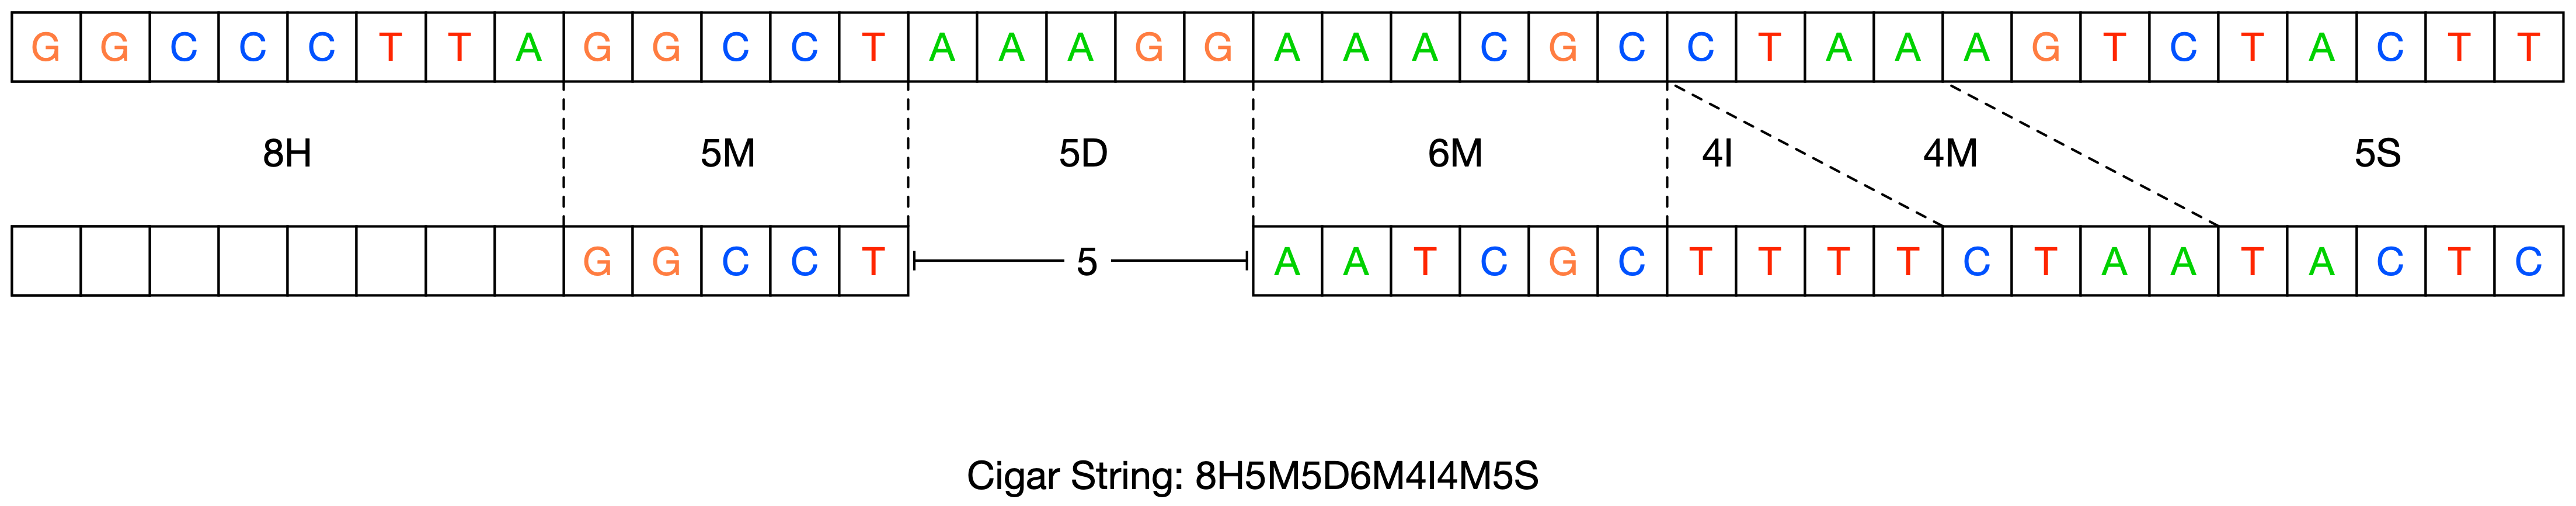
\includegraphics[scale=0.40]{cigar_string}
    \centering
    \caption {Example of an alignment CIGAR string.}
    \label{fig:main_body_cigar_string}
\end{figure}

If a co-linear set of seeds is not available, or the alignment score fails to reach the predetermined minimal score threshold then the read is emitted into the unmapped read stream with an appropriate flag set.

\bgroup
\def\arraystretch{1.5}
\begin{table}[!ht]
    \caption{Definition of $mapToReference()$}
    \label{tab:op_map_read_to_reference}
    {\begin{tabular}{l|p{12cm}}
    \toprule
    Inputs & \hangindent=1em$M_{raw} = \{m_i: m_i = (header, payload)\}$ where $m.payload = r = (s\_id, r\_id, b, q, f_p)$ as in \ref{eq:raw_read_message}. \\
    \cline{2-2}
    Operation & $mapToReference(r, ref\_id)$\\
    \cline{2-2}
    \multirow{2}{*}{Outputs} & \hangindent=1em$M_{aln} = \{m_i: m_i = (header, r)\} \text{ where } mr = (s\_id, r\_id, b, q, f_p, rname, pos, mapq, cigar, flags)$\\
    & \hangindent=1em $M_{unaln} = \{m_i: m_i = (header, r)\} \text{  where } r = (s\_id, r\_id, b, q, f_p, unmapped=true)$\\
    \bottomrule
    \end{tabular}}
\end{table}
\egroup


The reference pointed to by $ref_id$ when $mapToReference()$ is invoked consists of the typical data structures required by the FM Index i.e. the reference BWT, suffix array, occurrence array, as in \autocite{ferragina2000opportunistic}, but encoding both the forward and reverse complement of the reference sequence as in \autocite{Li2013} to produce the FMD index. Because the reference sequence is static, updated less frequently than once a year, the requisite data structures can be computed once offline and stored in secondary storage. During service initialization they are loaded in RAM and kept memory-resident for the duration of the operation of the service. Because, once computed, the reference index is read-only it can be accessed in a thread-safe manner by multiple concurrent threads without the need for explicit concurrency management. Because of the embarrassingly-parallel nature of read alignment this operation can be scaled up as necessary simply by adding servers, provided additional computational resources exist, and network capacity is not exhausted.

\paragraph{Read pair alignment to reference} - Since paired-end sequencing produces two reads that represent the opposite ends of a single molecule of approximately known size (known as insert size) it is possible to use knowledge about the insert size distribution along with corresponding pairs of reads to improve the quality of mapping for these reads, and even rescue mappings for reads that do not have a high quality unique mapping themselves but are anchored by a high quality mate. The mapping operation in this context proceeds similarly to the already described single read mapping but requires an input stream of read pairs along with a stream of sample QC metrics, including the empirical insert size distribution (as described in Section \ref{sec:main_body_read_qc_metrics}).

Depending on the result of the mapping operation for each read in a pair the output stream will contain pairs of reads of type \\
$r_{aln} = (s\_id, r\_id, b, q, f_p, rname, pos, mapq, cigar, flags)$\\
or \\
$r_{unaln} = (s\_id, r\_id, b, q, f_p, unmapped=true)$. 

\bgroup
\def\arraystretch{1.5}
\begin{table}[!ht]
    \caption{Definition of $mapPairToReference()$}
    \label{tab:op_map_pair_to_reference}
    {\begin{tabular}{l|p{12cm}}
    \toprule
    \multirow{2}{*}{Inputs} & \hangindent=1em$M_{pair} = \{m_i: m_i = (header, payload)\}$ where $m.payload = (r_1,r_2)$, and $r_i = (s\_id, r\_id, b, q, f_p)$ as in \ref{eq:raw_read_message}. \\
    & \hangindent=1em$M_{qc} = \{m_i: m_i = (header, payload)\}$ where $m.payload = (s\_id, \mu_{isd}, \sigma_{isd}^2, Q_{isd})$\\
    \cline{2-2}
    \multirow{2}{*}{Operations} & $mapPairToReference(r_1,r_2, ref\_id)$\\
    & $updateInsertSizeDistribution(s\_id,\mu_{isd}, \sigma_{isd}^2)$\\
    \cline{2-2}
    \multirow{2}{*}{Outputs} & \hangindent=1em$M_{aln} = \{m_i: m_i = (header, payload)\}$ where $m.payload = (r_1,r_2)$ and each read is of type $r_{aln}$\\
    & \hangindent=1em$M_{unaln} = \{m_i: m_i = (header, payload)\}$ where $m.payload = (r_1,r_2)$ and each read is of type $r_{aln}$ or $r_{unaln}$ depending on the outcome of mapping.\\
    \bottomrule
    \end{tabular}}
\end{table}
\egroup

In order to perform the $mapPairToReference()$ operation the service needs to have information about the insert size distribution for the sample the read pairs are originating from. It is notified with updated information about the insert size distribution by the $updateInsertSizeDistribution()$ operation which is subscribed to the appropriate message stream from the Read QC Service. This information is stored locally for each sample and may be cached. Assuming that the insert size distribution is approximately gaussian with mean $\mu_{isd}$ and variance $\sigma_{isd}^2$, which is the case for well-behaved samples, a scoring metric can be constructed that favours paired alignments that fall close to the expected insert size. This metric helps select among non-uniquely mapping reads. For instance, BWA-MEM uses the following metric:

\begin{equation}
    S_{ij}=S_i + S_j - \min{-a\log_4P(d_{ij}),U}
\end{equation}

Here $S_i$ and $S_j$ are the alignment scores for the individual reads in the pair obtained by single-end mapping via $mapToReference(r, ref\_id)$. $d_ij$ is the insert size implied by the mapping, $P(d_{i,j})$ is the probability of observing an insert size larger than $d$ under the assumption $D \sim \mathcal{N}(\mu_{isd}, \sigma_{isd}^2)$, $a$ is a matching score, and $U$ is a thresholding constant. Thus, given a set of possible mapping locations for each read in a pair, the joint mapping that maximizes the pairing metric is chosen.

$mapPairToReference()$ outputs read pairs to two output streams. If both reads are mapped successfully then they are output to the $M_{aln}$ stream. If at least one of two reads in a pair does not have a high quality mapping assigned through the paired mapping process, the pair is emitted through the $M_{unaln}$ stream.

Pairing information is vital to downstream variant calling because it can both help with fragment assembly, when reads are properly paired and mapped, and signal the location of potential structural variants when reads are not properly paired and mapped within expected distances.

\paragraph{Single read alignment to multiple references} -
\paragraph{Candidate haplotype alignment to reference} -
\paragraph{Single read alignment to list of alternative haplotypes} -
\paragraph{Single read split-alignment to reference} -


\subsection{Local Assembly}

\subsection{Simple SNP Calling}

\subsection{Assembly-based Variant Calling}

\subsection{Variant Filtering}

\subsection{Variant Annotation}

\subsection{Variant Output}

\hrule
Describe specific problems that need to be addressed by the system in a stream-based formulation - how to go from a collection of raw reads to a set of annotated variants: map reads, perform QC filtering, model loci, assemble alternative haplotypes, call variants, filter variants, annotate, produce output.  


\begin{itemize}
    \item Perform read QC
    \item Align reads to reference
    \item Collect read stream statistics
    \item Assemble local read contigs
    \item Model individual loci
    \item Call variants (maybe need to split by variant types)
    \item Genotype variants
    \item Filter variants
    \item Annotate variants
    \item Output variants
\end{itemize}




\section{Services of Rheos}

Provide a mapping from the domain-specific problems onto a particular implementation in the data streaming architecture. List services, their responsibilities, contracts, etc.

\begin{description}
    \item [Metadata] - Take in metadata related to patients, samples, files, etc. In: Metdata records, Out: ingestion confirmation events.
    \item [Read Streaming] - Take data from outside the system (file, web service, etc) and turn it into a standard stream. In: files, external streams, Out: internal read stream.
    \item [Read Persistence] - Store reads on disk, index. In: read stream, Out: persistence confirmation events.
    \item [Read Statistics] - Look at read stream and calculate various approximate stats of interest - insert size, GC-bias,  etc. In: read stream, Out: running stats of interest
    \item [QC] - Compute QC score for reads. In: reads, Out: reads with QC score
    \item [Read Filtering] - Filter out low quality reads based on configured parameters. In: reads with QC score, Out: filtered reads.
    \item [Read Mapping] - Align reads to reference genome. In: stream of reads, Out: streams of mapped, unmapped, split reads.
    \item [Local Assembly] - Local assembly of reads into candidate haplotypes. In: stream of aligned reads, Out: Updated haplotypes event.
    \item [Haplotype Persistence] - Storage and lookup of candidate haplotypes. In: stream of reads, Out: persistence confirmation events, stream of haplotypes.
    \item [Variant Calling] - Evaluate candidate haplotypes for presence of variation. In: haplotype update events, Out: variant update events.
    \item [Variant Persistence] - Storage and lookup of variants. In: stream of reads, Out: persistence confirmation events, stream of variants.
    \item [Genotyping] - Genotype variant sites. In: variant update stream, Out: genotype update events.
    \item [Variant Filtering] - Filter out low quality variants. In: stream of variants, Out: filtered stream of variants.
    \item [Variant annotation] - Annotate variants for functional impact. In: stream of variants, Out: stream of annotated variants.
    \item [Output variants] - Format variants for external output. In: stream of variants, Out: files, external variant stream.
    \item [Notification] - Notify the user when events of interest occur. In: any stream, Out: stream of notifications.
\end{description}

\section{Proof of concept implementation}

Describe actual implementation efforts. Focus on very basic use case (take already mapped reads from a file, turn them into a stream, use stream to call SNPs, maybe some Indels/SVs). Demonstrate some comparison metrics compared to other callers. Demonstrate some service-level metrics (throughput etc.)

\section{Conclusions}
Rheos is great!